% Options for packages loaded elsewhere
\PassOptionsToPackage{unicode}{hyperref}
\PassOptionsToPackage{hyphens}{url}
%
\documentclass[
]{article}
\usepackage{amsmath,amssymb}
\usepackage{iftex}
\ifPDFTeX
  \usepackage[T1]{fontenc}
  \usepackage[utf8]{inputenc}
  \usepackage{textcomp} % provide euro and other symbols
\else % if luatex or xetex
  \usepackage{unicode-math} % this also loads fontspec
  \defaultfontfeatures{Scale=MatchLowercase}
  \defaultfontfeatures[\rmfamily]{Ligatures=TeX,Scale=1}
\fi
\usepackage{lmodern}
\ifPDFTeX\else
  % xetex/luatex font selection
\fi
% Use upquote if available, for straight quotes in verbatim environments
\IfFileExists{upquote.sty}{\usepackage{upquote}}{}
\IfFileExists{microtype.sty}{% use microtype if available
  \usepackage[]{microtype}
  \UseMicrotypeSet[protrusion]{basicmath} % disable protrusion for tt fonts
}{}
\makeatletter
\@ifundefined{KOMAClassName}{% if non-KOMA class
  \IfFileExists{parskip.sty}{%
    \usepackage{parskip}
  }{% else
    \setlength{\parindent}{0pt}
    \setlength{\parskip}{6pt plus 2pt minus 1pt}}
}{% if KOMA class
  \KOMAoptions{parskip=half}}
\makeatother
\usepackage{xcolor}
\usepackage[margin=1in]{geometry}
\usepackage{color}
\usepackage{fancyvrb}
\newcommand{\VerbBar}{|}
\newcommand{\VERB}{\Verb[commandchars=\\\{\}]}
\DefineVerbatimEnvironment{Highlighting}{Verbatim}{commandchars=\\\{\}}
% Add ',fontsize=\small' for more characters per line
\usepackage{framed}
\definecolor{shadecolor}{RGB}{248,248,248}
\newenvironment{Shaded}{\begin{snugshade}}{\end{snugshade}}
\newcommand{\AlertTok}[1]{\textcolor[rgb]{0.94,0.16,0.16}{#1}}
\newcommand{\AnnotationTok}[1]{\textcolor[rgb]{0.56,0.35,0.01}{\textbf{\textit{#1}}}}
\newcommand{\AttributeTok}[1]{\textcolor[rgb]{0.13,0.29,0.53}{#1}}
\newcommand{\BaseNTok}[1]{\textcolor[rgb]{0.00,0.00,0.81}{#1}}
\newcommand{\BuiltInTok}[1]{#1}
\newcommand{\CharTok}[1]{\textcolor[rgb]{0.31,0.60,0.02}{#1}}
\newcommand{\CommentTok}[1]{\textcolor[rgb]{0.56,0.35,0.01}{\textit{#1}}}
\newcommand{\CommentVarTok}[1]{\textcolor[rgb]{0.56,0.35,0.01}{\textbf{\textit{#1}}}}
\newcommand{\ConstantTok}[1]{\textcolor[rgb]{0.56,0.35,0.01}{#1}}
\newcommand{\ControlFlowTok}[1]{\textcolor[rgb]{0.13,0.29,0.53}{\textbf{#1}}}
\newcommand{\DataTypeTok}[1]{\textcolor[rgb]{0.13,0.29,0.53}{#1}}
\newcommand{\DecValTok}[1]{\textcolor[rgb]{0.00,0.00,0.81}{#1}}
\newcommand{\DocumentationTok}[1]{\textcolor[rgb]{0.56,0.35,0.01}{\textbf{\textit{#1}}}}
\newcommand{\ErrorTok}[1]{\textcolor[rgb]{0.64,0.00,0.00}{\textbf{#1}}}
\newcommand{\ExtensionTok}[1]{#1}
\newcommand{\FloatTok}[1]{\textcolor[rgb]{0.00,0.00,0.81}{#1}}
\newcommand{\FunctionTok}[1]{\textcolor[rgb]{0.13,0.29,0.53}{\textbf{#1}}}
\newcommand{\ImportTok}[1]{#1}
\newcommand{\InformationTok}[1]{\textcolor[rgb]{0.56,0.35,0.01}{\textbf{\textit{#1}}}}
\newcommand{\KeywordTok}[1]{\textcolor[rgb]{0.13,0.29,0.53}{\textbf{#1}}}
\newcommand{\NormalTok}[1]{#1}
\newcommand{\OperatorTok}[1]{\textcolor[rgb]{0.81,0.36,0.00}{\textbf{#1}}}
\newcommand{\OtherTok}[1]{\textcolor[rgb]{0.56,0.35,0.01}{#1}}
\newcommand{\PreprocessorTok}[1]{\textcolor[rgb]{0.56,0.35,0.01}{\textit{#1}}}
\newcommand{\RegionMarkerTok}[1]{#1}
\newcommand{\SpecialCharTok}[1]{\textcolor[rgb]{0.81,0.36,0.00}{\textbf{#1}}}
\newcommand{\SpecialStringTok}[1]{\textcolor[rgb]{0.31,0.60,0.02}{#1}}
\newcommand{\StringTok}[1]{\textcolor[rgb]{0.31,0.60,0.02}{#1}}
\newcommand{\VariableTok}[1]{\textcolor[rgb]{0.00,0.00,0.00}{#1}}
\newcommand{\VerbatimStringTok}[1]{\textcolor[rgb]{0.31,0.60,0.02}{#1}}
\newcommand{\WarningTok}[1]{\textcolor[rgb]{0.56,0.35,0.01}{\textbf{\textit{#1}}}}
\usepackage{longtable,booktabs,array}
\usepackage{calc} % for calculating minipage widths
% Correct order of tables after \paragraph or \subparagraph
\usepackage{etoolbox}
\makeatletter
\patchcmd\longtable{\par}{\if@noskipsec\mbox{}\fi\par}{}{}
\makeatother
% Allow footnotes in longtable head/foot
\IfFileExists{footnotehyper.sty}{\usepackage{footnotehyper}}{\usepackage{footnote}}
\makesavenoteenv{longtable}
\usepackage{graphicx}
\makeatletter
\def\maxwidth{\ifdim\Gin@nat@width>\linewidth\linewidth\else\Gin@nat@width\fi}
\def\maxheight{\ifdim\Gin@nat@height>\textheight\textheight\else\Gin@nat@height\fi}
\makeatother
% Scale images if necessary, so that they will not overflow the page
% margins by default, and it is still possible to overwrite the defaults
% using explicit options in \includegraphics[width, height, ...]{}
\setkeys{Gin}{width=\maxwidth,height=\maxheight,keepaspectratio}
% Set default figure placement to htbp
\makeatletter
\def\fps@figure{htbp}
\makeatother
\setlength{\emergencystretch}{3em} % prevent overfull lines
\providecommand{\tightlist}{%
  \setlength{\itemsep}{0pt}\setlength{\parskip}{0pt}}
\setcounter{secnumdepth}{-\maxdimen} % remove section numbering
\ifLuaTeX
  \usepackage{selnolig}  % disable illegal ligatures
\fi
\usepackage{bookmark}
\IfFileExists{xurl.sty}{\usepackage{xurl}}{} % add URL line breaks if available
\urlstyle{same}
\hypersetup{
  hidelinks,
  pdfcreator={LaTeX via pandoc}}

\author{}
\date{\vspace{-2.5em}}

\begin{document}

\subsection{Generating simulated data}\label{generating-simulated-data}

The true model in this case is a logistic regression model.

Check: Can you understand the true data generating process by reading
the code?

\begin{Shaded}
\begin{Highlighting}[]
\CommentTok{\# Setting parameters}
\FunctionTok{set.seed}\NormalTok{(}\DecValTok{1}\NormalTok{)}
\CommentTok{\# Try changing some parameters}
\NormalTok{n }\OtherTok{\textless{}{-}} \DecValTok{500}
\NormalTok{p }\OtherTok{\textless{}{-}} \DecValTok{4}
\NormalTok{sparsity }\OtherTok{\textless{}{-}} \DecValTok{2}
\NormalTok{nonzero\_beta }\OtherTok{\textless{}{-}} 
  \FunctionTok{rep}\NormalTok{(}\DecValTok{1}\NormalTok{, sparsity) }\CommentTok{\# or e.g. runif(sparsity, min = {-}1, max = 1)}
\NormalTok{true\_beta }\OtherTok{\textless{}{-}} \FunctionTok{c}\NormalTok{(nonzero\_beta, }\FunctionTok{rep}\NormalTok{(}\DecValTok{0}\NormalTok{, p }\SpecialCharTok{{-}}\NormalTok{ sparsity))}
\NormalTok{class\_shift }\OtherTok{\textless{}{-}} \FloatTok{2.5} \CommentTok{\# change this}
\end{Highlighting}
\end{Shaded}

The \textbar\textgreater{} operator is called the pipe operator. It
allows you to pass the output of one function directly as the input to
another function in a more readable and streamlined way. It is similar
in functionality to the \%\textgreater\% operator.

select(y, num\_range(``x.'', 1:4)): select columns with names that
contain the prefix ``x.'' followed by a number within a specified range.

Purpose of class\_shift: control the balance of the classes. Larger
shift leads to larger mu, then leads to higher proportion of positive
class (class 1).

\begin{Shaded}
\begin{Highlighting}[]
\CommentTok{\# Generating simulated data}
\NormalTok{X }\OtherTok{\textless{}{-}} \FunctionTok{matrix}\NormalTok{(}\FunctionTok{rnorm}\NormalTok{(n}\SpecialCharTok{*}\NormalTok{p), }\AttributeTok{nrow =}\NormalTok{ n)}
\NormalTok{mu }\OtherTok{\textless{}{-}}\NormalTok{ class\_shift }\SpecialCharTok{+}\NormalTok{ X }\SpecialCharTok{\%*\%}\NormalTok{ true\_beta  }\CommentTok{\#z = XW+b }
\NormalTok{px }\OtherTok{\textless{}{-}} \FunctionTok{exp}\NormalTok{(mu)}\SpecialCharTok{/}\NormalTok{(}\DecValTok{1}\SpecialCharTok{+}\FunctionTok{exp}\NormalTok{(mu))}
\NormalTok{Y }\OtherTok{\textless{}{-}} \FunctionTok{rbinom}\NormalTok{(n, }\DecValTok{1}\NormalTok{, }\AttributeTok{prob =}\NormalTok{ px)}
\NormalTok{train\_ld }\OtherTok{\textless{}{-}} \FunctionTok{data.frame}\NormalTok{(}\AttributeTok{y =} \FunctionTok{as.factor}\NormalTok{(Y), }\AttributeTok{x =}\NormalTok{ X)}
\NormalTok{train\_ld }\SpecialCharTok{|\textgreater{}}
  \FunctionTok{select}\NormalTok{(y, }\FunctionTok{num\_range}\NormalTok{(}\StringTok{"x."}\NormalTok{, }\DecValTok{1}\SpecialCharTok{:}\DecValTok{4}\NormalTok{)) }\SpecialCharTok{|\textgreater{}}
  \FunctionTok{ggpairs}\NormalTok{(}\AttributeTok{progress =}\NormalTok{ F)}
\end{Highlighting}
\end{Shaded}

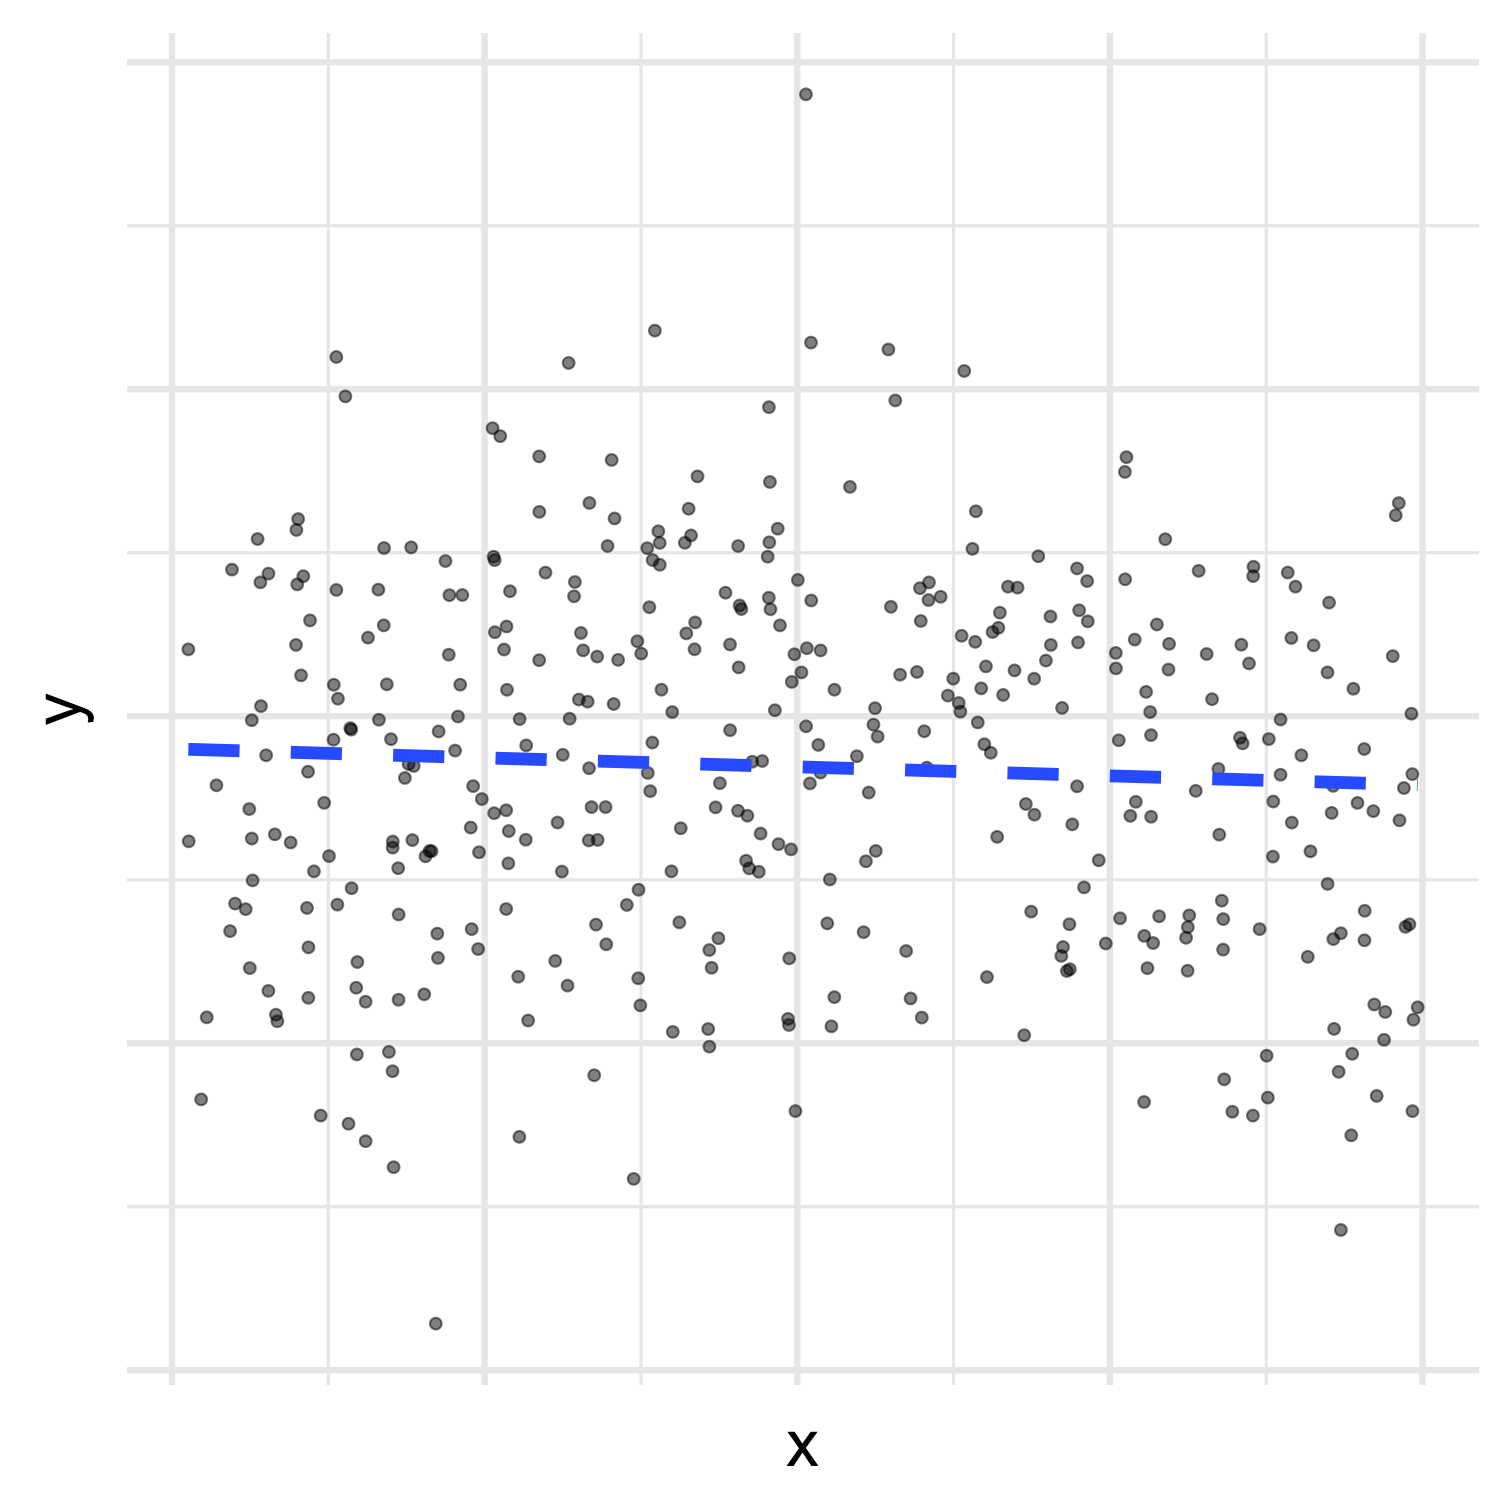
\includegraphics{classification_complete_files/figure-latex/unnamed-chunk-2-1.pdf}

Check: Do these plots fit with your understanding of the true data
generating process?

\begin{Shaded}
\begin{Highlighting}[]
\CommentTok{\# Class (im)balance}
\FunctionTok{table}\NormalTok{(train\_ld}\SpecialCharTok{$}\NormalTok{y)}
\end{Highlighting}
\end{Shaded}

\begin{verbatim}
## 
##   0   1 
##  74 426
\end{verbatim}

\begin{Shaded}
\begin{Highlighting}[]
\NormalTok{train\_ld }\SpecialCharTok{|\textgreater{}} \FunctionTok{count}\NormalTok{(y)}
\end{Highlighting}
\end{Shaded}

\begin{verbatim}
##   y   n
## 1 0  74
## 2 1 426
\end{verbatim}

\textbf{Question}: What would the accuracy be for a classifier that
always predicts the most common class?

\begin{Shaded}
\begin{Highlighting}[]
\NormalTok{const\_yhat\_success }\OtherTok{\textless{}{-}} \FunctionTok{mean}\NormalTok{(train\_ld}\SpecialCharTok{$}\NormalTok{y }\SpecialCharTok{==} \DecValTok{1}\NormalTok{)}
\FunctionTok{max}\NormalTok{(const\_yhat\_success, }\DecValTok{1} \SpecialCharTok{{-}}\NormalTok{ const\_yhat\_success) }\CommentTok{\# this equals to 426/500=0.852, but only on training data, meaningless.}
\end{Highlighting}
\end{Shaded}

\begin{verbatim}
## [1] 0.852
\end{verbatim}

\subsection{Logistic regression model}\label{logistic-regression-model}

\subsubsection{Coefficients}\label{coefficients}

\begin{Shaded}
\begin{Highlighting}[]
\FunctionTok{c}\NormalTok{(class\_shift, true\_beta)}
\end{Highlighting}
\end{Shaded}

\begin{verbatim}
## [1] 2.5 1.0 1.0 0.0 0.0
\end{verbatim}

\begin{Shaded}
\begin{Highlighting}[]
\NormalTok{fit\_glm }\OtherTok{\textless{}{-}} \FunctionTok{glm}\NormalTok{(y }\SpecialCharTok{\textasciitilde{}}\NormalTok{ ., }\AttributeTok{family =} \FunctionTok{binomial}\NormalTok{(), }\AttributeTok{data =}\NormalTok{ train\_ld)}
\NormalTok{fit\_glm}
\end{Highlighting}
\end{Shaded}

\begin{verbatim}
## 
## Call:  glm(formula = y ~ ., family = binomial(), data = train_ld)
## 
## Coefficients:
## (Intercept)          x.1          x.2          x.3          x.4  
##     2.48089      1.19239      1.04222      0.11820     -0.04386  
## 
## Degrees of Freedom: 499 Total (i.e. Null);  495 Residual
## Null Deviance:       419.2 
## Residual Deviance: 317.6     AIC: 327.6
\end{verbatim}

\begin{Shaded}
\begin{Highlighting}[]
\NormalTok{fit\_glm }\SpecialCharTok{|\textgreater{}} \FunctionTok{ggcoef}\NormalTok{()}
\end{Highlighting}
\end{Shaded}

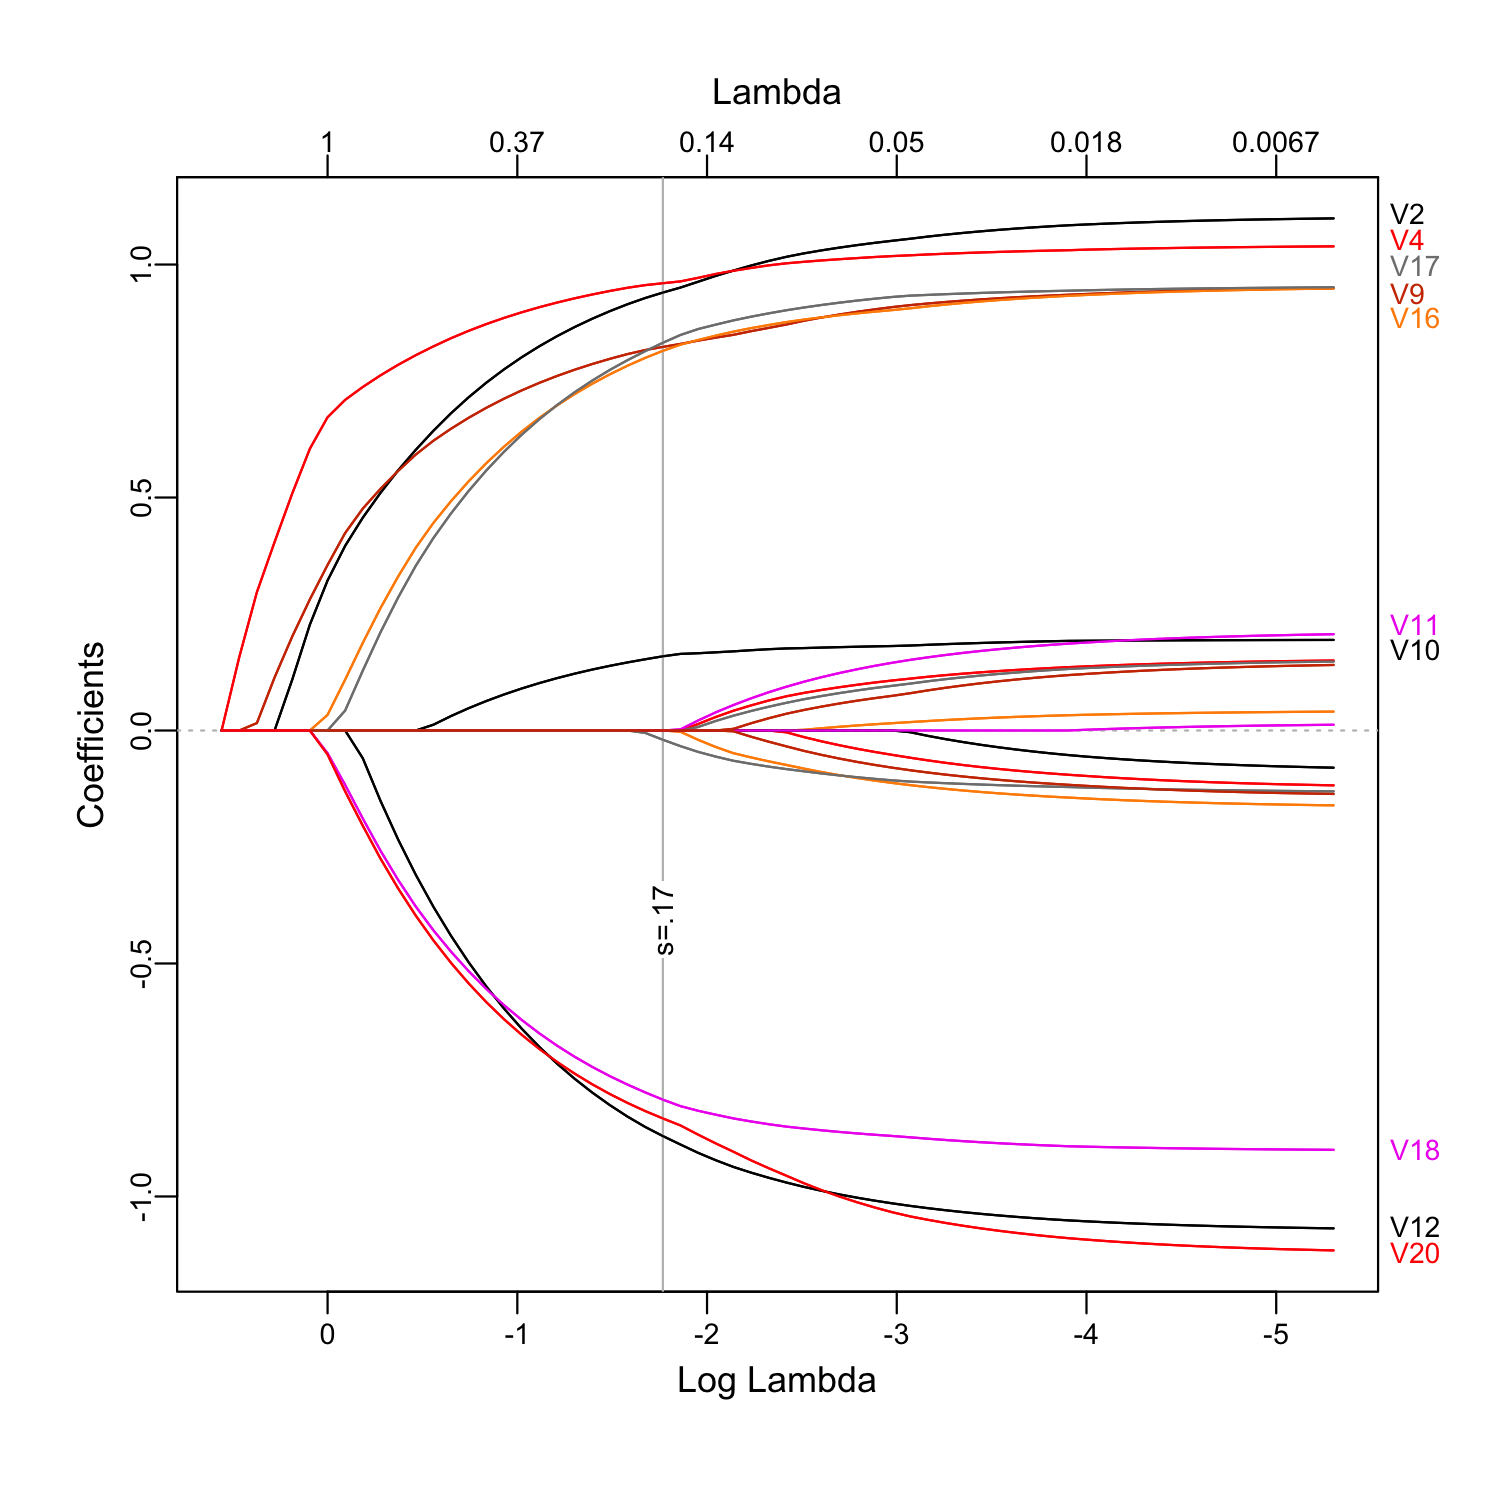
\includegraphics{classification_complete_files/figure-latex/unnamed-chunk-6-1.pdf}

Coefficients on the odds scale:

The coefficients from the glm model are the coefficients of the logits,
which is exponential of the odds. We can the exponential of the
coefficients such that we can observe how they change odds. For example,
\(\beta_1=1.19\), this means we increase x1 by one unit, logits
\(\log(\frac{p}{1-p})\) will increase by 1.19. In the following
coefficient for x1 is 3.29, which means we increase x1 by one unit, odds
ratio will be 3.29 greater.

\begin{Shaded}
\begin{Highlighting}[]
\NormalTok{fit\_glm }\OtherTok{\textless{}{-}} \FunctionTok{glm}\NormalTok{(y }\SpecialCharTok{\textasciitilde{}}\NormalTok{ ., }\AttributeTok{family =} \FunctionTok{binomial}\NormalTok{(), }\AttributeTok{data =}\NormalTok{ train\_ld)}
\NormalTok{fit\_glm }\SpecialCharTok{|\textgreater{}} 
  \FunctionTok{tidy}\NormalTok{(}\AttributeTok{exponentiate =} \ConstantTok{TRUE}\NormalTok{) }\SpecialCharTok{|\textgreater{}}\NormalTok{ knitr}\SpecialCharTok{::}\FunctionTok{kable}\NormalTok{()}
\end{Highlighting}
\end{Shaded}

\begin{longtable}[]{@{}lrrrr@{}}
\toprule\noalign{}
term & estimate & std.error & statistic & p.value \\
\midrule\noalign{}
\endhead
\bottomrule\noalign{}
\endlastfoot
(Intercept) & 11.9518723 & 0.2067843 & 11.9974661 & 0.0000000 \\
x.1 & 3.2949620 & 0.1704925 & 6.9938266 & 0.0000000 \\
x.2 & 2.8355109 & 0.1622098 & 6.4251500 & 0.0000000 \\
x.3 & 1.1254655 & 0.1456378 & 0.8115803 & 0.4170325 \\
x.4 & 0.9570916 & 0.1344844 & -0.3261060 & 0.7443442 \\
\end{longtable}

\subsubsection{Predictions}\label{predictions}

\begin{Shaded}
\begin{Highlighting}[]
\NormalTok{fit\_glm\_predictions }\OtherTok{\textless{}{-}} \FunctionTok{augment}\NormalTok{(fit\_glm, }\AttributeTok{type.predict =} \StringTok{"response"}\NormalTok{)}
\NormalTok{fit\_glm\_predictions }\SpecialCharTok{|\textgreater{}} \FunctionTok{pull}\NormalTok{(.fitted) }\SpecialCharTok{|\textgreater{}} \FunctionTok{mean}\NormalTok{() }\CommentTok{\#take out the column named .fitted and calculate the mean.}
\end{Highlighting}
\end{Shaded}

\begin{verbatim}
## [1] 0.852
\end{verbatim}

\begin{Shaded}
\begin{Highlighting}[]
\FunctionTok{mean}\NormalTok{(fit\_glm\_predictions}\SpecialCharTok{$}\NormalTok{.fitted)}
\end{Highlighting}
\end{Shaded}

\begin{verbatim}
## [1] 0.852
\end{verbatim}

\textbf{Question}: Does this number look familiar? Why?

\textbf{Answer}: It's the proportion of the majority class that we saw
before. Any other value here would indicate an overall bias in the
predictions of the model.

\begin{Shaded}
\begin{Highlighting}[]
\CommentTok{\# Note: the event\_level option is currently required because}
\CommentTok{\# of a mismatch between glm() and yardstick}
\NormalTok{fit\_glm\_predictions }\SpecialCharTok{|\textgreater{}}
  \FunctionTok{roc\_curve}\NormalTok{(}\AttributeTok{truth =}\NormalTok{ y, .fitted,}
            \AttributeTok{event\_level =} \StringTok{"second"}\NormalTok{) }\SpecialCharTok{|\textgreater{}}
  \FunctionTok{autoplot}\NormalTok{()}
\end{Highlighting}
\end{Shaded}

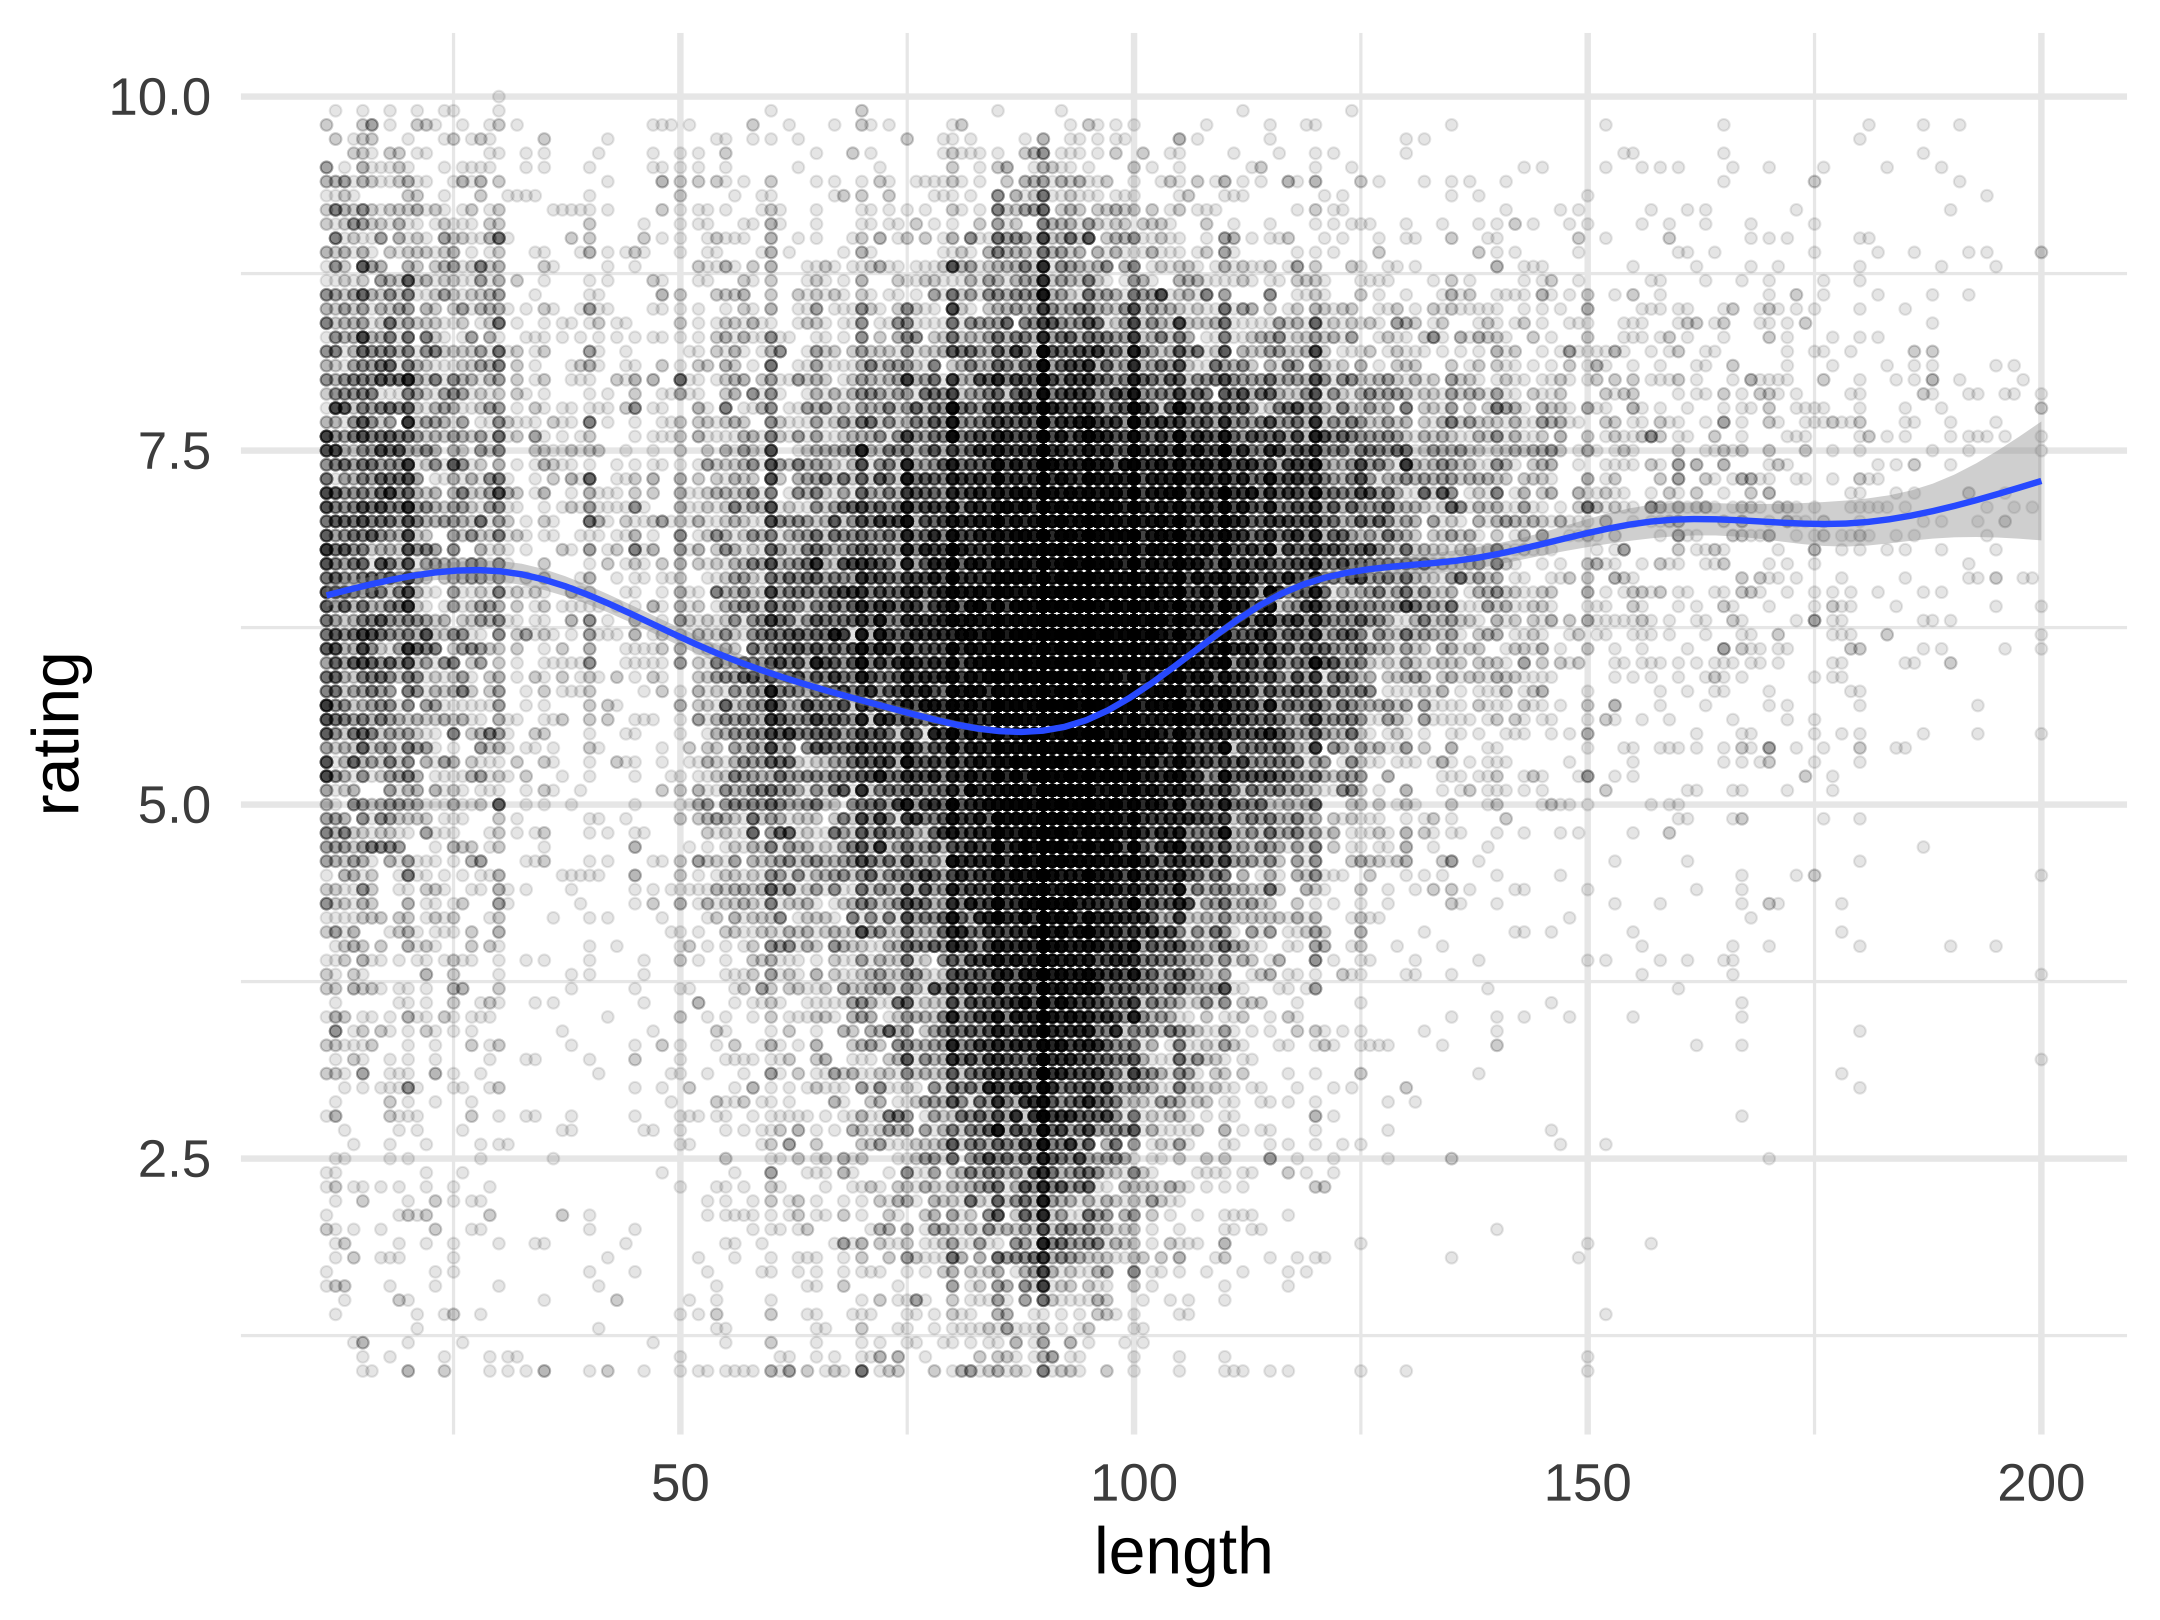
\includegraphics{classification_complete_files/figure-latex/unnamed-chunk-10-1.pdf}
ROC curve: TPR against FPR, consisting of choosing different levels of
threshold. At (0,0), the threshold is 1, which means we choose all to be
negative, hence TPR=FPR=0; At (1,1), the threshold is 0, which means we
vote all positive, then TPR=FPR=1.

\textbf{Note}: When a classification model outputs class probabilities
or numeric scores these can be converted into classifications by setting
thresholds or cutoffs. If we keep the model fixed but change the cutoff,
we can achieve different trade-offs between false positives and false
negatives (or specificity and sensitivity, precision and recall,
etc--these are just other names). Plots like this \texttt{roc\_curve}
(see also \texttt{?pr\_curve}) show all the possible trade-off values
for one model.

\textbf{Question}: Using curves like this how can we compare different
models? Give at least two suggestions.

\textbf{Answer}: We could compare at a specific point on the curve, for
example if that point corresponds to a certain false positive rate that
has some practical or domain-specific importance (e.g.~regulations). Or
we could compute the area under the curves, e.g.~using the
\texttt{roc\_auc} function.

Classify at several different thresholds

\begin{Shaded}
\begin{Highlighting}[]
\CommentTok{\# Note: true and predicted classes must use same}
\CommentTok{\# label names, hence the factor(as.numeric()) }
\NormalTok{higher\_cutoff }\OtherTok{\textless{}{-}}\NormalTok{ const\_yhat\_success }\SpecialCharTok{+}\NormalTok{ .}\DecValTok{05}
\NormalTok{confusion\_matrix\_higher }\OtherTok{\textless{}{-}}
\NormalTok{  fit\_glm\_predictions }\SpecialCharTok{|\textgreater{}}
  \FunctionTok{mutate}\NormalTok{(}\AttributeTok{yhat =} \FunctionTok{factor}\NormalTok{(}\FunctionTok{as.numeric}\NormalTok{(.fitted }\SpecialCharTok{\textgreater{}}\NormalTok{ higher\_cutoff))) }\SpecialCharTok{|\textgreater{}}
  \FunctionTok{conf\_mat}\NormalTok{(}\AttributeTok{truth =}\NormalTok{ y, }\AttributeTok{estimate =}\NormalTok{ yhat)}
\end{Highlighting}
\end{Shaded}

\begin{Shaded}
\begin{Highlighting}[]
\NormalTok{lower\_cutoff }\OtherTok{\textless{}{-}}\NormalTok{ .}\DecValTok{2}
\NormalTok{confusion\_matrix\_lower }\OtherTok{\textless{}{-}}
\NormalTok{  fit\_glm\_predictions }\SpecialCharTok{|\textgreater{}}
  \FunctionTok{mutate}\NormalTok{(}\AttributeTok{yhat =} \FunctionTok{factor}\NormalTok{(}\FunctionTok{as.numeric}\NormalTok{(.fitted }\SpecialCharTok{\textgreater{}}\NormalTok{ lower\_cutoff))) }\SpecialCharTok{|\textgreater{}}
  \FunctionTok{conf\_mat}\NormalTok{(}\AttributeTok{truth =}\NormalTok{ y, }\AttributeTok{estimate =}\NormalTok{ yhat)}
\end{Highlighting}
\end{Shaded}

\begin{Shaded}
\begin{Highlighting}[]
\NormalTok{confusion\_matrix\_higher}
\end{Highlighting}
\end{Shaded}

\begin{verbatim}
##           Truth
## Prediction   0   1
##          0  65 164
##          1   9 262
\end{verbatim}

\begin{Shaded}
\begin{Highlighting}[]
\NormalTok{confusion\_matrix\_lower}
\end{Highlighting}
\end{Shaded}

\begin{verbatim}
##           Truth
## Prediction   0   1
##          0   0   2
##          1  74 424
\end{verbatim}

\begin{Shaded}
\begin{Highlighting}[]
\NormalTok{confusion\_matrix\_higher }\SpecialCharTok{|\textgreater{}} \FunctionTok{autoplot}\NormalTok{(}\AttributeTok{type =} \StringTok{"heatmap"}\NormalTok{)}
\end{Highlighting}
\end{Shaded}

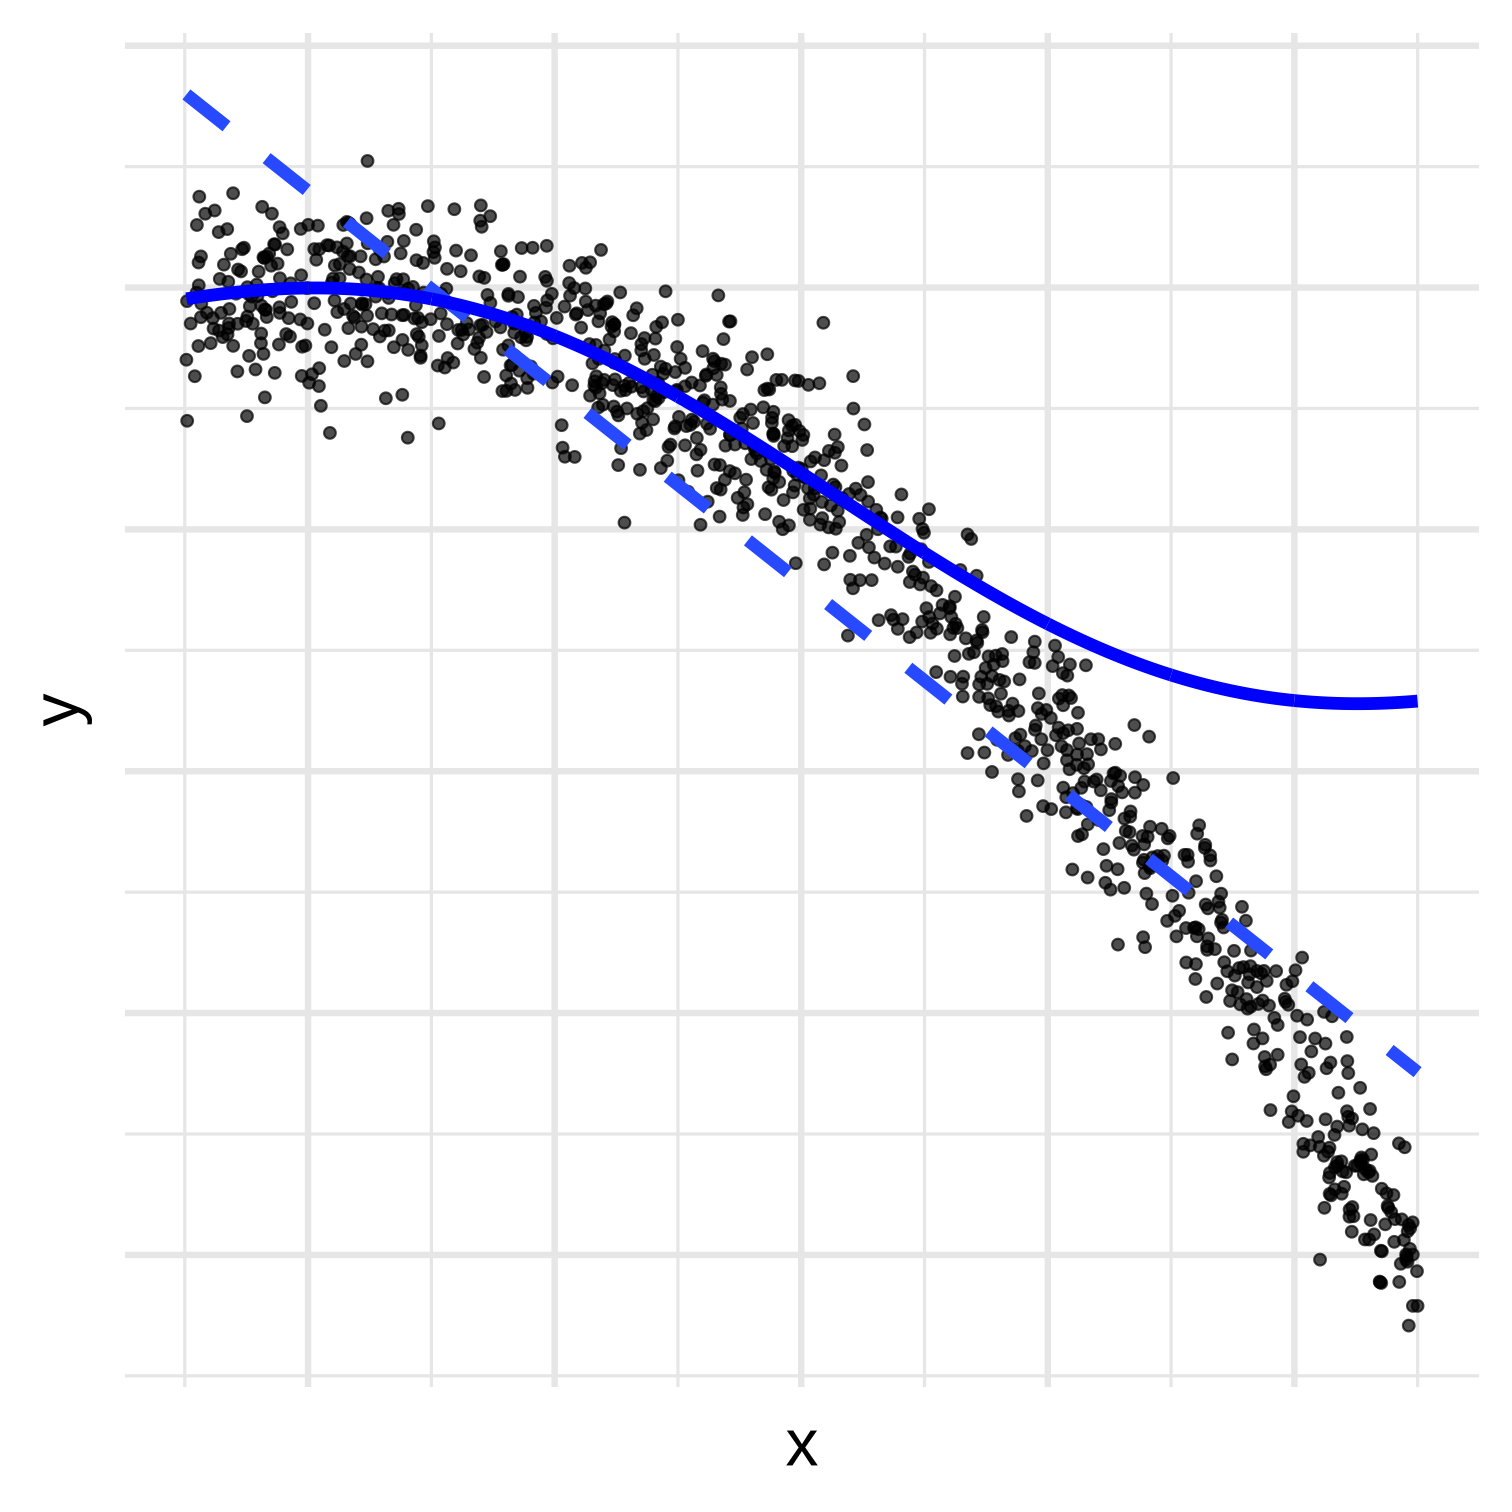
\includegraphics{classification_complete_files/figure-latex/unnamed-chunk-15-1.pdf}

\begin{Shaded}
\begin{Highlighting}[]
\NormalTok{confusion\_matrix\_lower }\SpecialCharTok{|\textgreater{}} \FunctionTok{autoplot}\NormalTok{(}\AttributeTok{type =} \StringTok{"heatmap"}\NormalTok{) }\CommentTok{\#almost all predictions are positive}
\end{Highlighting}
\end{Shaded}

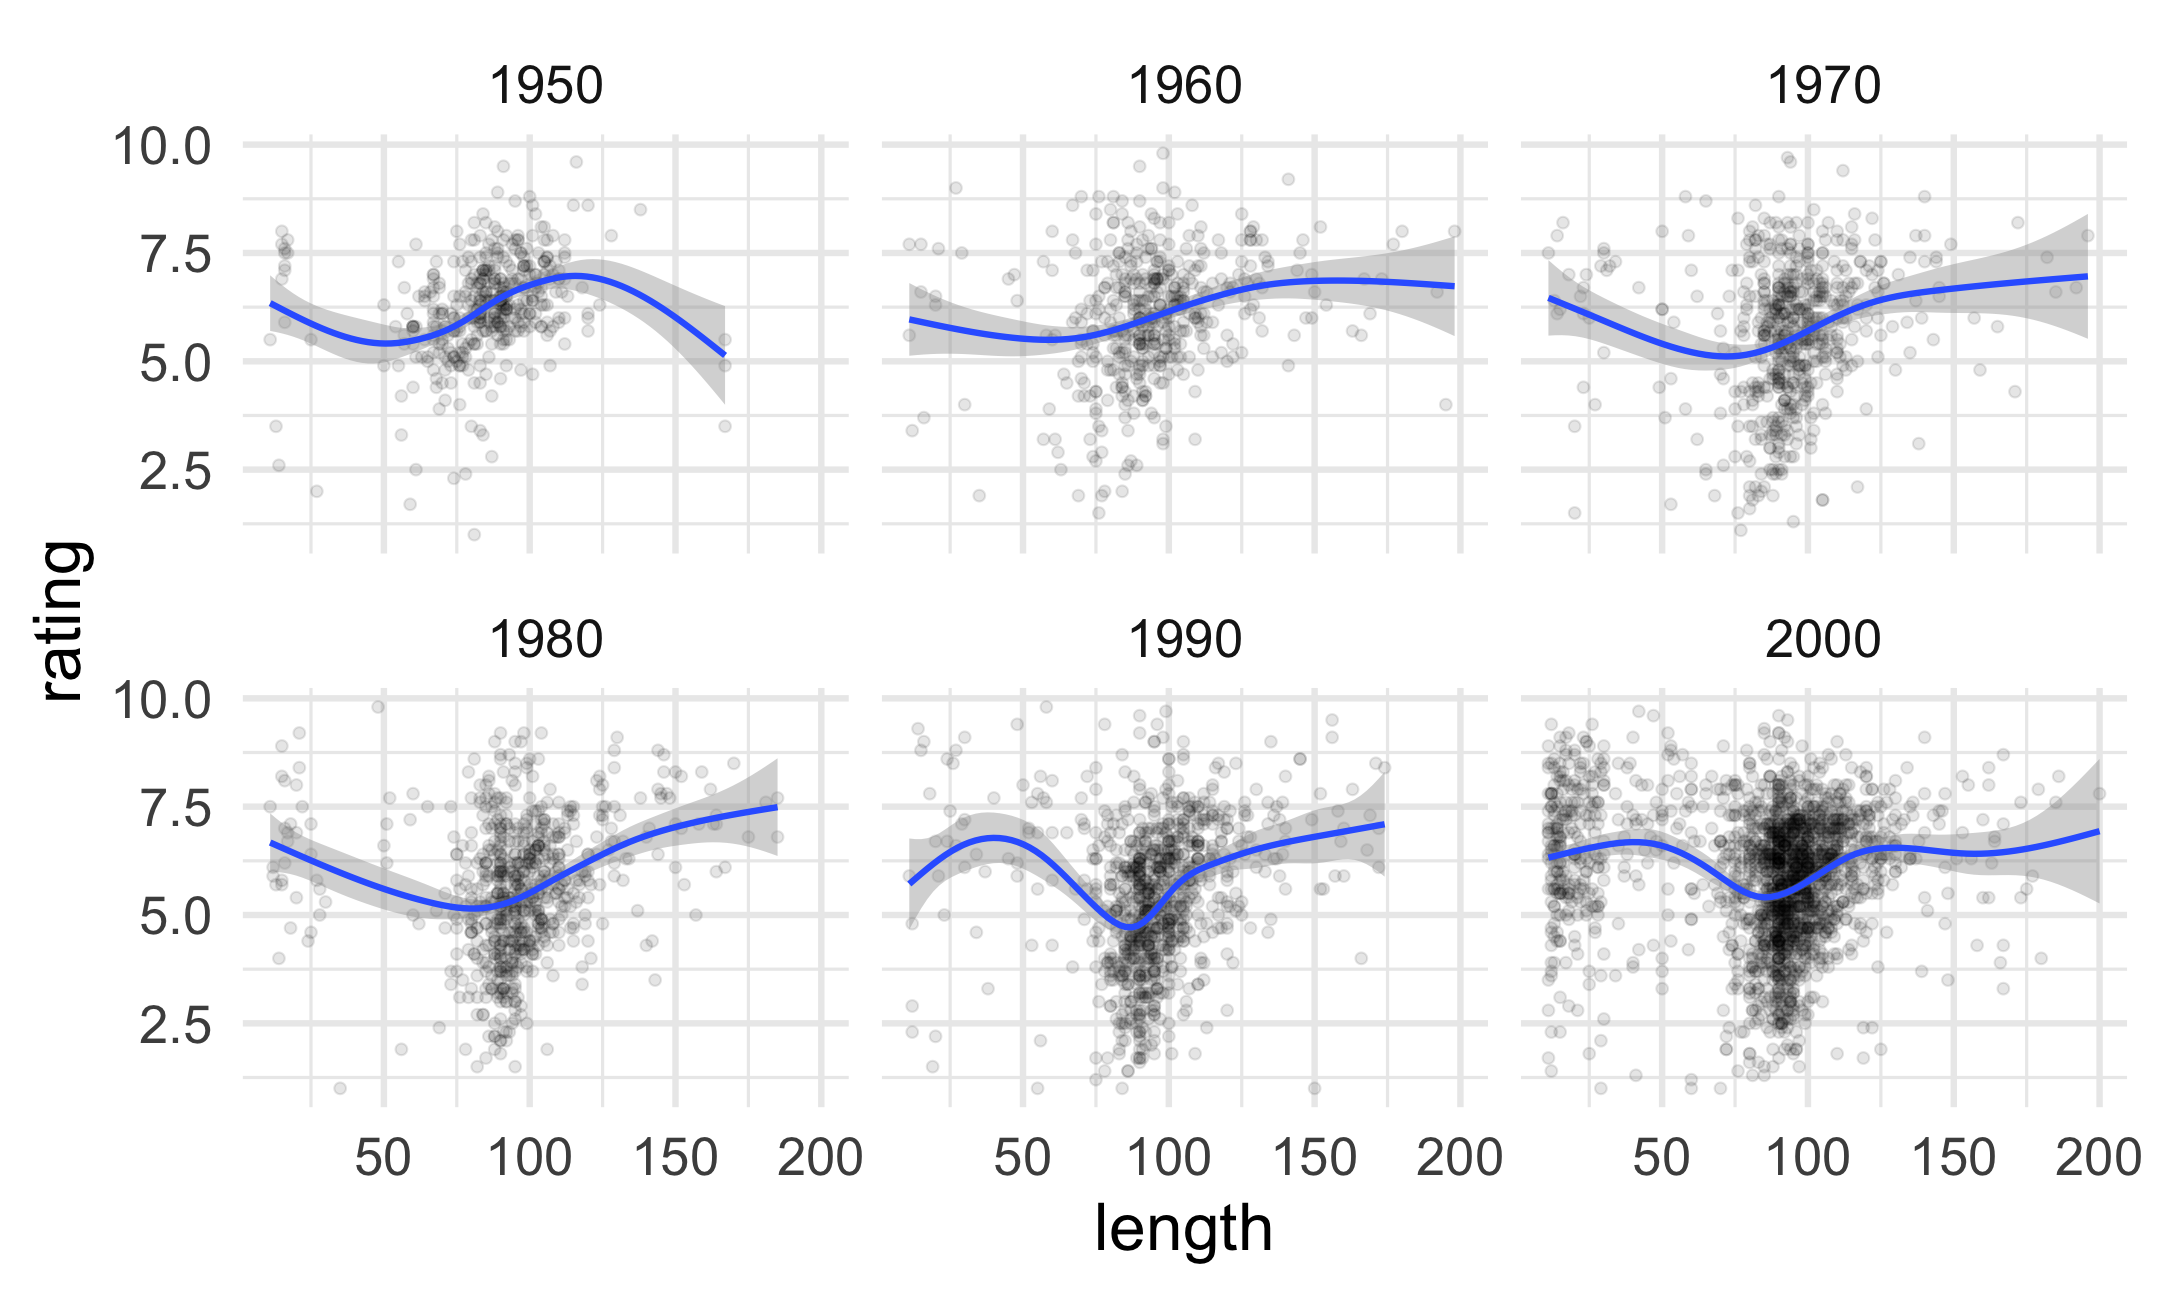
\includegraphics{classification_complete_files/figure-latex/unnamed-chunk-16-1.pdf}

Comparing across various metrics:

\begin{Shaded}
\begin{Highlighting}[]
\NormalTok{higher\_summary }\OtherTok{\textless{}{-}} \FunctionTok{summary}\NormalTok{(confusion\_matrix\_higher) }\SpecialCharTok{|\textgreater{}}
  \FunctionTok{mutate}\NormalTok{(}\AttributeTok{higher =}\NormalTok{ .estimate) }\SpecialCharTok{|\textgreater{}}
  \FunctionTok{select}\NormalTok{(.metric, higher)}
\NormalTok{lower\_summary }\OtherTok{\textless{}{-}} \FunctionTok{summary}\NormalTok{(confusion\_matrix\_lower) }\SpecialCharTok{|\textgreater{}}
  \FunctionTok{mutate}\NormalTok{(}\AttributeTok{lower =}\NormalTok{ .estimate) }\SpecialCharTok{|\textgreater{}}
  \FunctionTok{select}\NormalTok{(lower)}
\FunctionTok{cbind}\NormalTok{(higher\_summary, lower\_summary) }\SpecialCharTok{|\textgreater{}}
\NormalTok{  knitr}\SpecialCharTok{::}\FunctionTok{kable}\NormalTok{()}
\end{Highlighting}
\end{Shaded}

\begin{longtable}[]{@{}lrr@{}}
\toprule\noalign{}
.metric & higher & lower \\
\midrule\noalign{}
\endhead
\bottomrule\noalign{}
\endlastfoot
accuracy & 0.6540000 & 0.8480000 \\
kap & 0.2645058 & -0.0078506 \\
sens & 0.8783784 & 0.0000000 \\
spec & 0.6150235 & 0.9953052 \\
ppv & 0.2838428 & 0.0000000 \\
npv & 0.9667897 & 0.8514056 \\
mcc & 0.3516568 & -0.0264126 \\
j\_index & 0.4934019 & -0.0046948 \\
bal\_accuracy & 0.7467009 & 0.4976526 \\
detection\_prevalence & 0.4580000 & 0.0040000 \\
precision & 0.2838428 & 0.0000000 \\
recall & 0.8783784 & 0.0000000 \\
f\_meas & 0.4290429 & 0.0000000 \\
\end{longtable}

Accuracy benefits from a lower threshold, since the data is very
imbalanced toward positive class. So a lower threshold will vote toward
the positive class.

Note the \texttt{accuracy}, for example, which is the proportion of data
where the predicted class and true class are equal.

\subsubsection{Sub-sampling for class
balance}\label{sub-sampling-for-class-balance}

choose the number of positive samples to be the same as negative samples

\begin{Shaded}
\begin{Highlighting}[]
\NormalTok{rare\_class\_size }\OtherTok{\textless{}{-}} \FunctionTok{min}\NormalTok{(}\FunctionTok{table}\NormalTok{(train\_ld}\SpecialCharTok{$}\NormalTok{y))}
\NormalTok{train\_subsampled }\OtherTok{\textless{}{-}}\NormalTok{ train\_ld }\SpecialCharTok{|\textgreater{}}
  \FunctionTok{group\_by}\NormalTok{(y) }\SpecialCharTok{|\textgreater{}}
  \FunctionTok{sample\_n}\NormalTok{(rare\_class\_size) }\SpecialCharTok{|\textgreater{}}
  \FunctionTok{ungroup}\NormalTok{()}
  
\NormalTok{fit\_glm\_subs }\OtherTok{\textless{}{-}} \FunctionTok{glm}\NormalTok{(y }\SpecialCharTok{\textasciitilde{}}\NormalTok{ ., }\AttributeTok{family =} \FunctionTok{binomial}\NormalTok{(), }\AttributeTok{data =}\NormalTok{ train\_subsampled)}
\end{Highlighting}
\end{Shaded}

Does this change coefficients or inferences about them?

\begin{Shaded}
\begin{Highlighting}[]
\FunctionTok{cbind}\NormalTok{(}
  \FunctionTok{tidy}\NormalTok{(fit\_glm) }\SpecialCharTok{|\textgreater{}} \FunctionTok{select}\NormalTok{(term, estimate, std.error),}
  \FunctionTok{tidy}\NormalTok{(fit\_glm\_subs) }\SpecialCharTok{|\textgreater{}} \FunctionTok{select}\NormalTok{(estimate, std.error)) }\SpecialCharTok{|\textgreater{}}
\NormalTok{  knitr}\SpecialCharTok{::}\FunctionTok{kable}\NormalTok{()}
\end{Highlighting}
\end{Shaded}

\begin{longtable}[]{@{}lrrrr@{}}
\toprule\noalign{}
term & estimate & std.error & estimate & std.error \\
\midrule\noalign{}
\endhead
\bottomrule\noalign{}
\endlastfoot
(Intercept) & 2.4808879 & 0.2067843 & 0.8869130 & 0.2734060 \\
x.1 & 1.1923946 & 0.1704925 & 1.6250092 & 0.2957344 \\
x.2 & 1.0422221 & 0.1622098 & 1.1683666 & 0.2551454 \\
x.3 & 0.1181967 & 0.1456378 & 0.2936595 & 0.2475284 \\
x.4 & -0.0438562 & 0.1344844 & 0.0915651 & 0.1980801 \\
\end{longtable}

\begin{Shaded}
\begin{Highlighting}[]
\NormalTok{fit\_glm}
\end{Highlighting}
\end{Shaded}

\begin{verbatim}
## 
## Call:  glm(formula = y ~ ., family = binomial(), data = train_ld)
## 
## Coefficients:
## (Intercept)          x.1          x.2          x.3          x.4  
##     2.48089      1.19239      1.04222      0.11820     -0.04386  
## 
## Degrees of Freedom: 499 Total (i.e. Null);  495 Residual
## Null Deviance:       419.2 
## Residual Deviance: 317.6     AIC: 327.6
\end{verbatim}

\begin{Shaded}
\begin{Highlighting}[]
\NormalTok{fit\_glm\_subs}
\end{Highlighting}
\end{Shaded}

\begin{verbatim}
## 
## Call:  glm(formula = y ~ ., family = binomial(), data = train_subsampled)
## 
## Coefficients:
## (Intercept)          x.1          x.2          x.3          x.4  
##     0.88691      1.62501      1.16837      0.29366      0.09157  
## 
## Degrees of Freedom: 147 Total (i.e. Null);  143 Residual
## Null Deviance:       205.2 
## Residual Deviance: 135.2     AIC: 145.2
\end{verbatim}

\textbf{Note}: With a smaller sample size, the balanced training data
gives us larger \texttt{std.errors} for our estimates. (Wider confident
intervals, larger p-values).

\begin{Shaded}
\begin{Highlighting}[]
\NormalTok{fit\_glm\_subs\_predictions }\OtherTok{\textless{}{-}} \FunctionTok{augment}\NormalTok{(fit\_glm\_subs, }\AttributeTok{type.predict =} \StringTok{"response"}\NormalTok{)}
\NormalTok{fit\_glm\_subs\_predictions }\SpecialCharTok{|\textgreater{}} \FunctionTok{pull}\NormalTok{(.fitted) }\SpecialCharTok{|\textgreater{}} \FunctionTok{mean}\NormalTok{()}
\end{Highlighting}
\end{Shaded}

\begin{verbatim}
## [1] 0.5
\end{verbatim}

Training data classes are balanced so the predictions are also balanced.

\begin{Shaded}
\begin{Highlighting}[]
\CommentTok{\# Note: the event\_level option is currently required because}
\CommentTok{\# of a mismatch between glm() and yardstick}
\NormalTok{fit\_glm\_subs\_predictions }\SpecialCharTok{|\textgreater{}}
  \FunctionTok{roc\_curve}\NormalTok{(}\AttributeTok{truth =}\NormalTok{ y, .fitted,}
            \AttributeTok{event\_level =} \StringTok{"second"}\NormalTok{) }\SpecialCharTok{|\textgreater{}}
  \FunctionTok{autoplot}\NormalTok{()}
\end{Highlighting}
\end{Shaded}

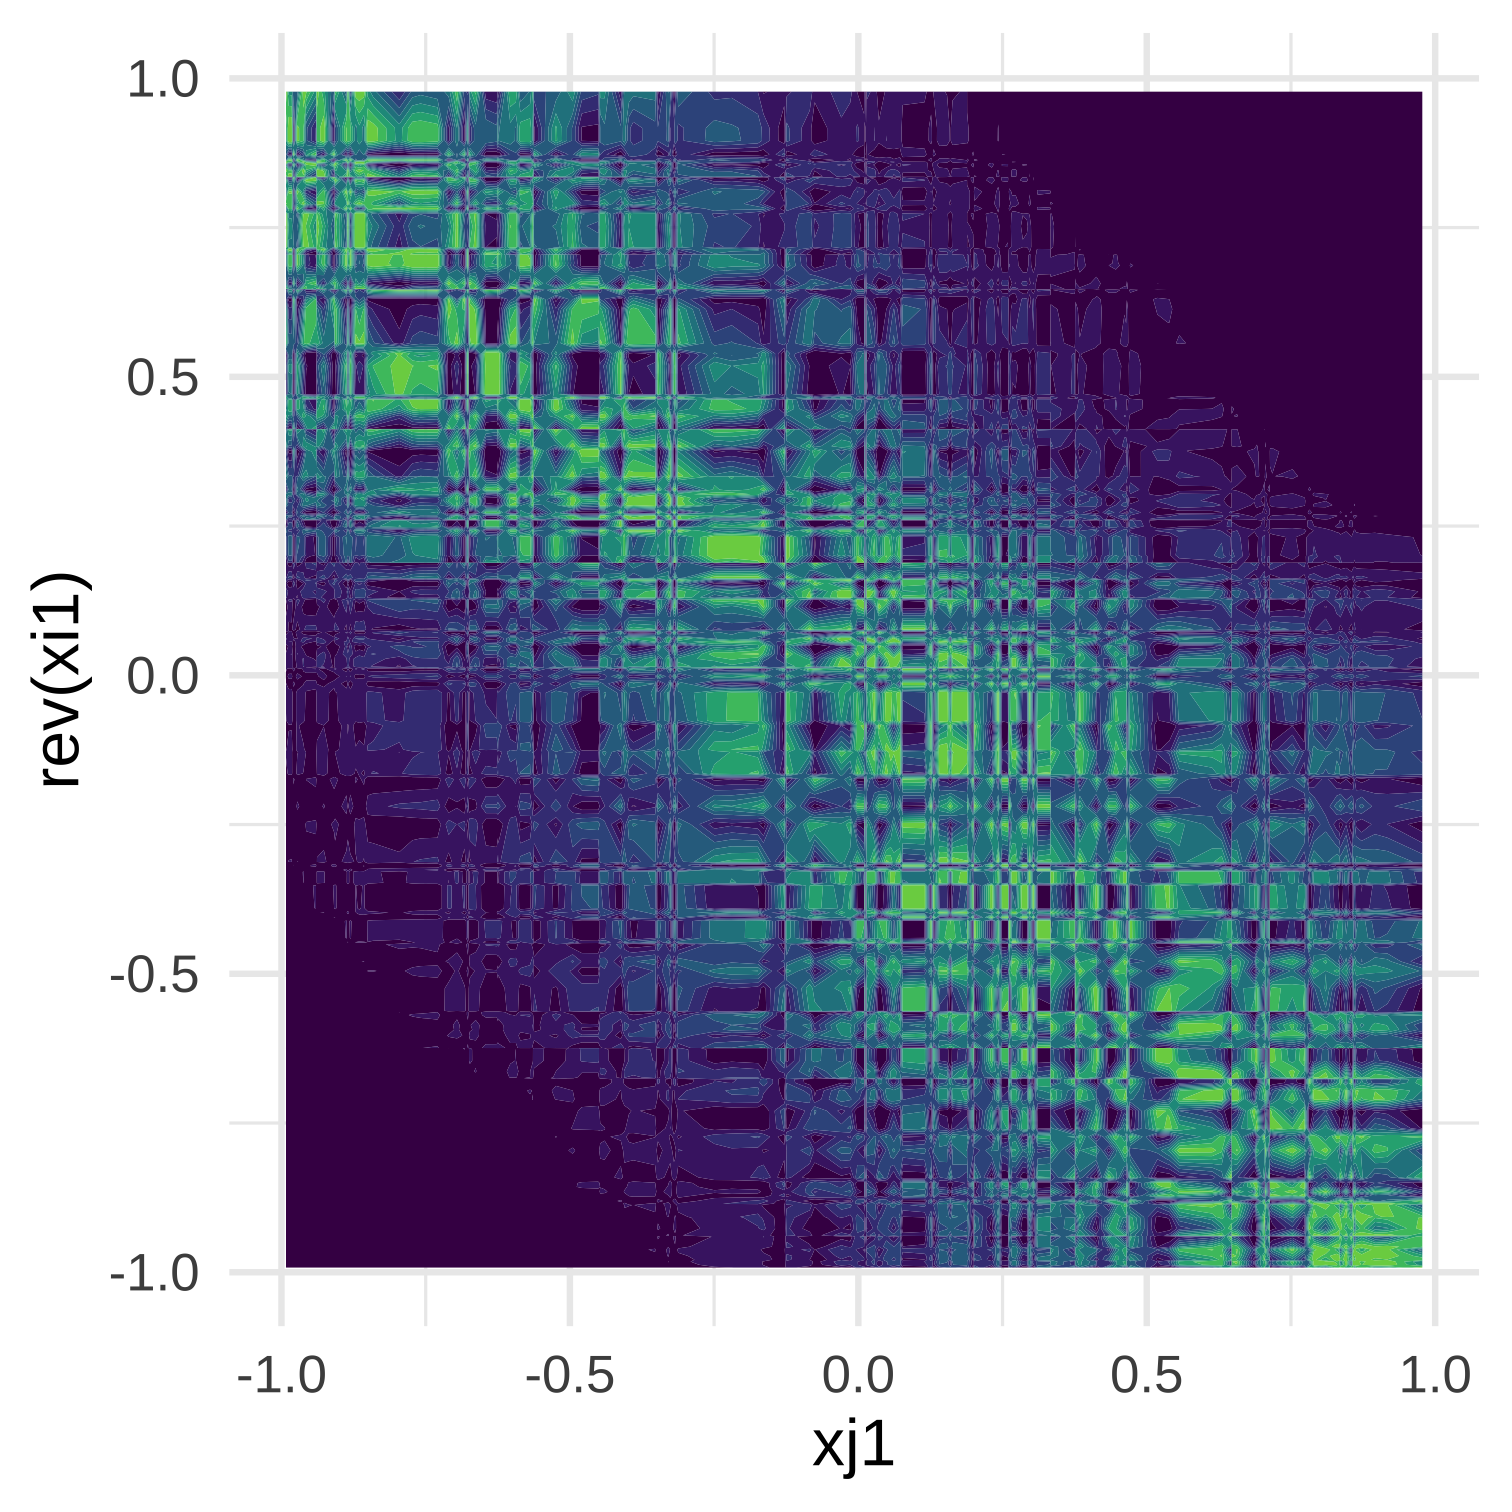
\includegraphics{classification_complete_files/figure-latex/unnamed-chunk-22-1.pdf}

Classify at several different thresholds

\begin{Shaded}
\begin{Highlighting}[]
\CommentTok{\# Note: true and predicted classes must use same}
\CommentTok{\# label names, hence the factor(as.numeric()) }
\NormalTok{higher\_cutoff }\OtherTok{\textless{}{-}}\NormalTok{ const\_yhat\_success }\SpecialCharTok{+}\NormalTok{ .}\DecValTok{05}
\NormalTok{confusion\_matrix\_subs\_higher }\OtherTok{\textless{}{-}}
\NormalTok{  fit\_glm\_subs\_predictions }\SpecialCharTok{|\textgreater{}}
  \FunctionTok{mutate}\NormalTok{(}\AttributeTok{yhat =} \FunctionTok{factor}\NormalTok{(}\FunctionTok{as.numeric}\NormalTok{(.fitted }\SpecialCharTok{\textgreater{}}\NormalTok{ higher\_cutoff))) }\SpecialCharTok{|\textgreater{}}
  \FunctionTok{conf\_mat}\NormalTok{(}\AttributeTok{truth =}\NormalTok{ y, }\AttributeTok{estimate =}\NormalTok{ yhat)}
\end{Highlighting}
\end{Shaded}

\begin{Shaded}
\begin{Highlighting}[]
\NormalTok{lower\_cutoff }\OtherTok{\textless{}{-}}\NormalTok{ .}\DecValTok{2}
\NormalTok{confusion\_matrix\_subs\_lower }\OtherTok{\textless{}{-}}
\NormalTok{  fit\_glm\_subs\_predictions }\SpecialCharTok{|\textgreater{}}
  \FunctionTok{mutate}\NormalTok{(}\AttributeTok{yhat =} \FunctionTok{factor}\NormalTok{(}\FunctionTok{as.numeric}\NormalTok{(.fitted }\SpecialCharTok{\textgreater{}}\NormalTok{ lower\_cutoff))) }\SpecialCharTok{|\textgreater{}}
  \FunctionTok{conf\_mat}\NormalTok{(}\AttributeTok{truth =}\NormalTok{ y, }\AttributeTok{estimate =}\NormalTok{ yhat)}
\end{Highlighting}
\end{Shaded}

\begin{Shaded}
\begin{Highlighting}[]
\NormalTok{confusion\_matrix\_subs\_higher}
\end{Highlighting}
\end{Shaded}

\begin{verbatim}
##           Truth
## Prediction  0  1
##          0 74 48
##          1  0 26
\end{verbatim}

\begin{Shaded}
\begin{Highlighting}[]
\NormalTok{confusion\_matrix\_subs\_lower}
\end{Highlighting}
\end{Shaded}

\begin{verbatim}
##           Truth
## Prediction  0  1
##          0 35  4
##          1 39 70
\end{verbatim}

\begin{Shaded}
\begin{Highlighting}[]
\NormalTok{confusion\_matrix\_subs\_higher }\SpecialCharTok{|\textgreater{}} \FunctionTok{autoplot}\NormalTok{(}\AttributeTok{type =} \StringTok{"heatmap"}\NormalTok{)}
\end{Highlighting}
\end{Shaded}

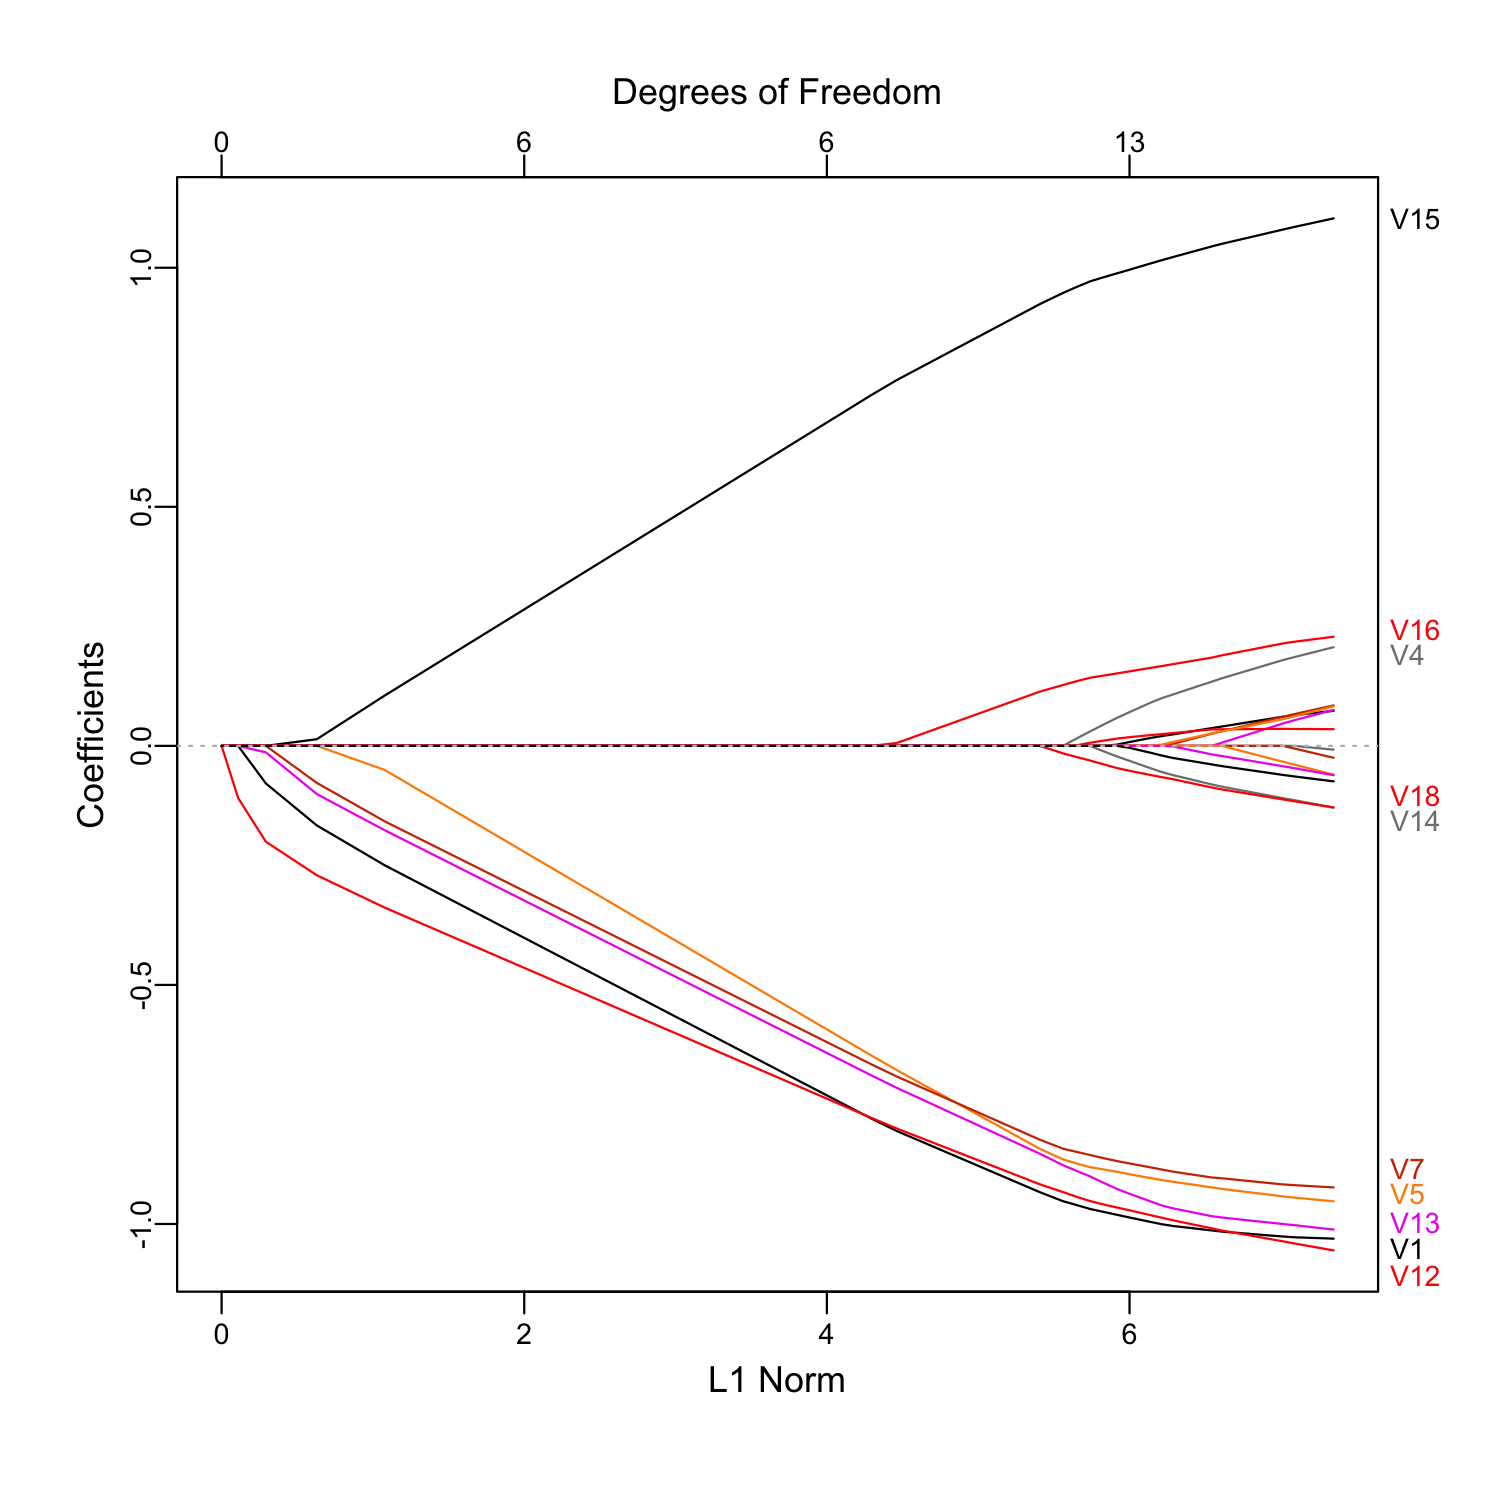
\includegraphics{classification_complete_files/figure-latex/unnamed-chunk-27-1.pdf}

\begin{Shaded}
\begin{Highlighting}[]
\NormalTok{confusion\_matrix\_subs\_lower }\SpecialCharTok{|\textgreater{}} \FunctionTok{autoplot}\NormalTok{(}\AttributeTok{type =} \StringTok{"heatmap"}\NormalTok{)}
\end{Highlighting}
\end{Shaded}

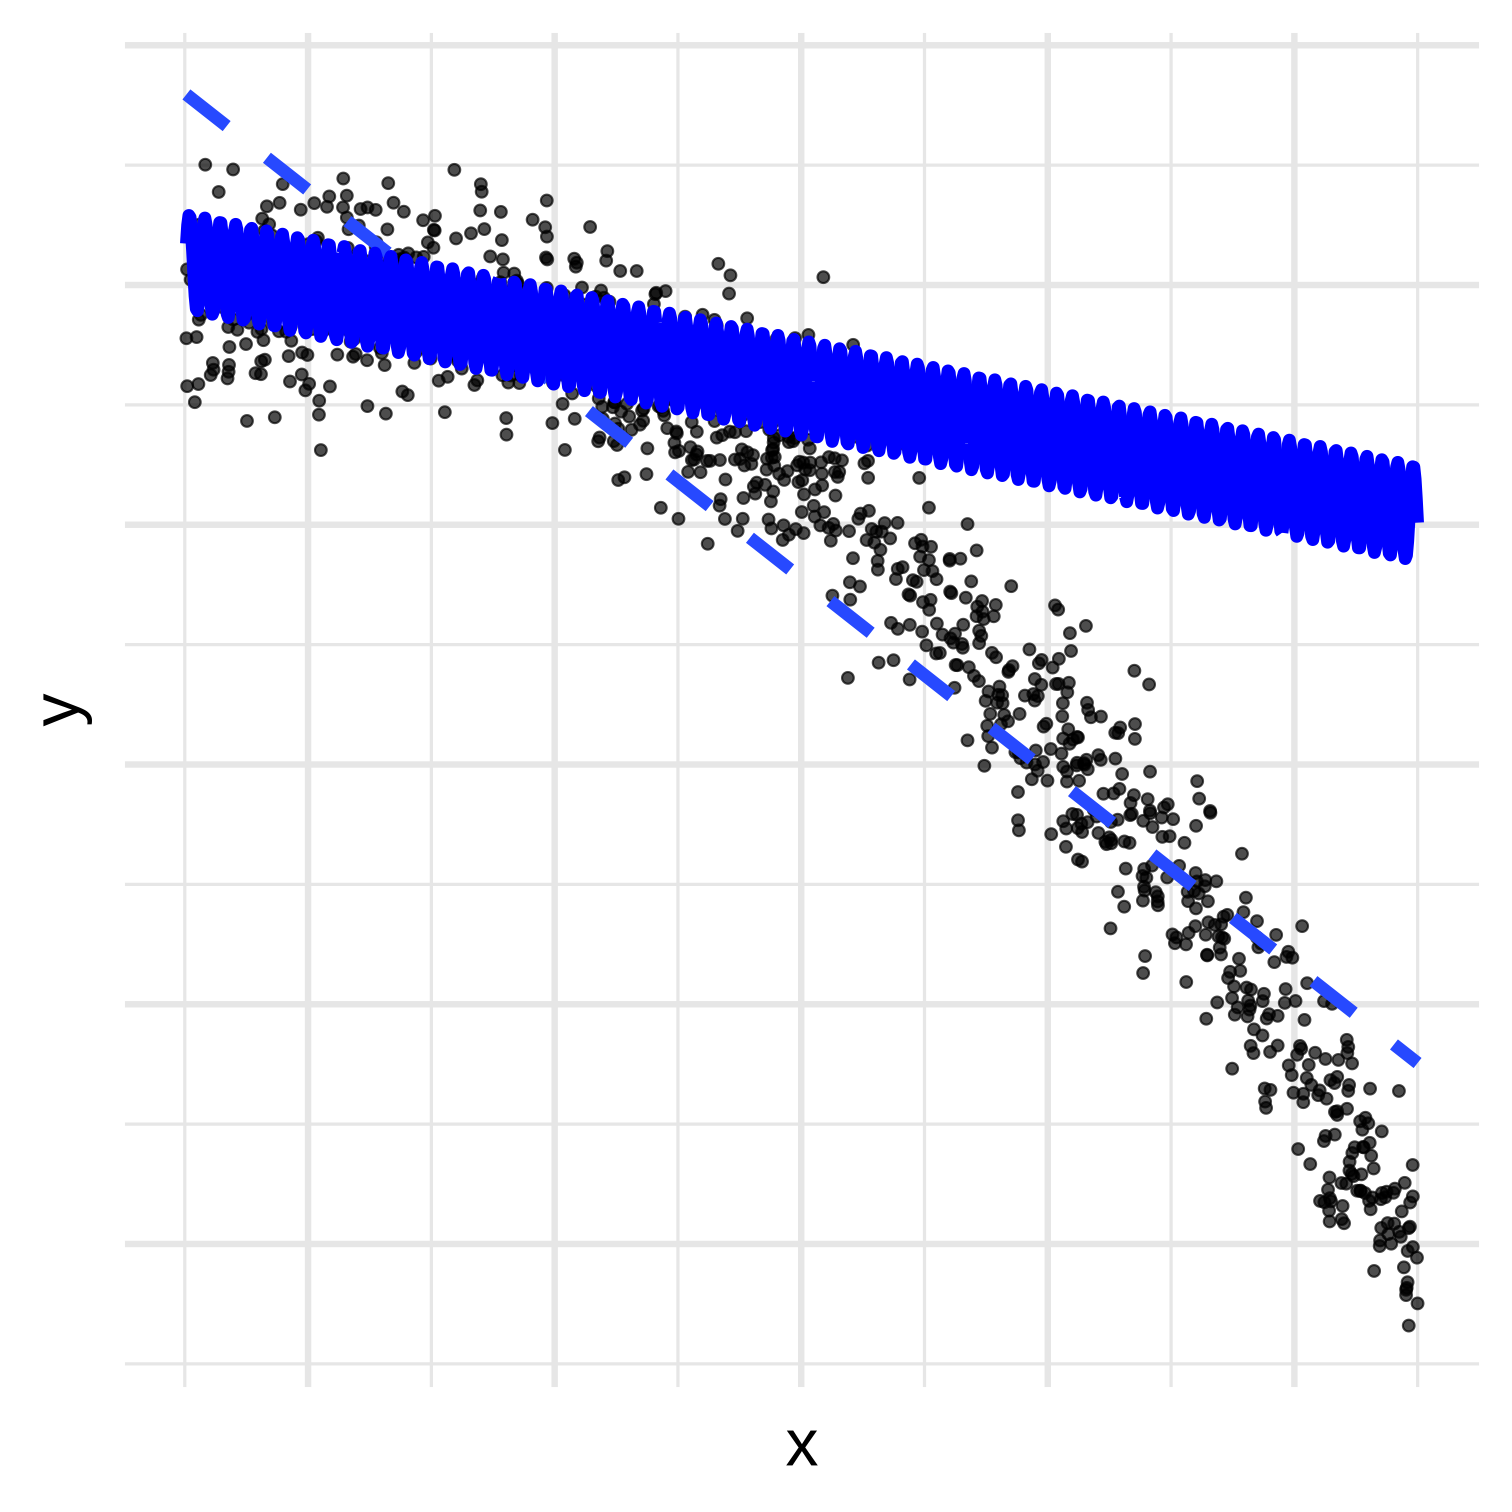
\includegraphics{classification_complete_files/figure-latex/unnamed-chunk-28-1.pdf}

Comparing across various metrics:

\begin{Shaded}
\begin{Highlighting}[]
\NormalTok{higher\_subs\_summary }\OtherTok{\textless{}{-}} \FunctionTok{summary}\NormalTok{(confusion\_matrix\_subs\_higher) }\SpecialCharTok{|\textgreater{}}
  \FunctionTok{mutate}\NormalTok{(}\AttributeTok{higher =}\NormalTok{ .estimate) }\SpecialCharTok{|\textgreater{}}
  \FunctionTok{select}\NormalTok{(.metric, higher)}
\NormalTok{lower\_subs\_summary }\OtherTok{\textless{}{-}} \FunctionTok{summary}\NormalTok{(confusion\_matrix\_subs\_lower) }\SpecialCharTok{|\textgreater{}}
  \FunctionTok{mutate}\NormalTok{(}\AttributeTok{lower =}\NormalTok{ .estimate) }\SpecialCharTok{|\textgreater{}}
  \FunctionTok{select}\NormalTok{(lower)}
\NormalTok{metrics }\OtherTok{\textless{}{-}} \FunctionTok{c}\NormalTok{(}\StringTok{"accuracy"}\NormalTok{, }\StringTok{"bal\_accuracy"}\NormalTok{) }\CommentTok{\#, "precision", "recall")}
\FunctionTok{rbind}\NormalTok{(}
\FunctionTok{cbind}\NormalTok{(higher\_summary, lower\_summary) }\SpecialCharTok{|\textgreater{}}
  \FunctionTok{filter}\NormalTok{(.metric }\SpecialCharTok{\%in\%}\NormalTok{ metrics) }\SpecialCharTok{|\textgreater{}}
  \FunctionTok{mutate}\NormalTok{(}\AttributeTok{subsampled =} \ConstantTok{FALSE}\NormalTok{),}
\FunctionTok{cbind}\NormalTok{(higher\_subs\_summary, lower\_subs\_summary) }\SpecialCharTok{|\textgreater{}}
  \FunctionTok{filter}\NormalTok{(.metric }\SpecialCharTok{\%in\%}\NormalTok{ metrics) }\SpecialCharTok{|\textgreater{}}
  \FunctionTok{mutate}\NormalTok{(}\AttributeTok{subsampled =} \ConstantTok{TRUE}\NormalTok{)) }\SpecialCharTok{|\textgreater{}}
\NormalTok{  knitr}\SpecialCharTok{::}\FunctionTok{kable}\NormalTok{()}
\end{Highlighting}
\end{Shaded}

\begin{longtable}[]{@{}lrrl@{}}
\toprule\noalign{}
.metric & higher & lower & subsampled \\
\midrule\noalign{}
\endhead
\bottomrule\noalign{}
\endlastfoot
accuracy & 0.6540000 & 0.8480000 & FALSE \\
bal\_accuracy & 0.7467009 & 0.4976526 & FALSE \\
accuracy & 0.6756757 & 0.7094595 & TRUE \\
bal\_accuracy & 0.6756757 & 0.7094595 & TRUE \\
\end{longtable}

\textbf{Question}: Suppose we have trained a model on data that was
subsampled to create class balance. Then we choose classification
cutoffs to achieve a desired trade-off between precision/recall (or
false positives and false negatives), and we do this still while using
the subsampled training data. What will happen if we start using that
model to classify data from a new or full dataset that hasn't been
subsampled? \textbf{Answer}: Predictions on imbalanced data will achieve
a different trade-off between false positives and false negatives. To
calibrate this we would need to choose a different classification
threshold that works on imbalanced data.

In a word: What if we train on a balanced dataset and predict on an
imbalanced dataset? Answer: adjust the threshold according to the
dominating class. If positive class dominates, increase the threshold;
otherwise decrease the threshold. Or we can use some other metrics which
are not so sensitive to the class imbalance, such as F1 score or
balanced accuracy.

\section{Logistic Regression}\label{logistic-regression}

\section{1. Sigmoid Function}\label{sigmoid-function}

The logistic function, also known as the \textbf{sigmoid function}, is
used to model the relationship between input features and the
probability of the positive class:

\[
\sigma(z) = \frac{1}{1 + e^{-z}}
\]

where \(z\) is the linear combination of the input features:

\[
z = \mathbf{w}^T \mathbf{x}
\]

\begin{itemize}
\tightlist
\item
  \(\mathbf{w}\): Weights of the model.
\item
  \(\mathbf{x}\): Feature vector.
\end{itemize}

The output of the logistic function is a value between \textbf{0 and 1},
representing the predicted probability of the positive class.

\section{2. Log-Odds and Linear
Relationship}\label{log-odds-and-linear-relationship}

The \textbf{log-odds} (or \textbf{logit}) is the logarithm of the odds
of the positive class. In logistic regression, the log-odds is modeled
as a linear function of the input features:

\[
\text{logit}(p) = \log\left( \frac{p}{1 - p} \right) = \mathbf{w}^T \mathbf{x}
\]

where \(p\) is the predicted probability of the positive class.

\section{3. Cost Function and Maximum Likelihood
Estimation}\label{cost-function-and-maximum-likelihood-estimation}

The goal of logistic regression is to find the optimal parameters
(weights and bias) that minimize the prediction error. Instead of using
\textbf{Mean Squared Error}, logistic regression uses the
\textbf{logistic loss} or \textbf{cross-entropy loss} function, which is
defined as:

\[
C(\mathbf{w}) = -\frac{1}{m} \sum_{i=1}^m \left[ y^{(i)} \log(\hat{y}^{(i)}) + (1 - y^{(i)}) \log(1 - \hat{y}^{(i)}) \right]
\]

The cost function represents the \textbf{negative log-likelihood} of the
data given the model parameters.

\section{4. Maximum Likelihood
Derivation}\label{maximum-likelihood-derivation}

To estimate the parameters, we use \textbf{Maximum Likelihood Estimation
(MLE)}. The likelihood function for logistic regression is:

\[
L(\mathbf{w}) = \prod_{i=1}^m \left( \hat{y}^{(i)} \right)^{y^{(i)}} \left( 1 - \hat{y}^{(i)} \right)^{1 - y^{(i)}}
\]

The \textbf{log-likelihood} is obtained by taking the logarithm of the
likelihood function:

\[
\ell(\mathbf{w}) = \sum_{i=1}^m \left[ y^{(i)} \log(\hat{y}^{(i)}) + (1 - y^{(i)}) \log(1 - \hat{y}^{(i)}) \right]
\]

The \textbf{negative log-likelihood} is equivalent to the cost function,
which we aim to minimize.

Question: why there may be problems for logistic regression in a
well-classified data?

the log-likelihood function is maximized when the predicted
probabilities approach 0 or 1 for all data points, which is only
possible if the coefficients approach infinity. Have a look at the
log-likelihood function, it is maximized either when \(\hat y=0\) or
\(\hat y=1\). The predicted probability is \[
P(\hat y =1) =\frac{1}{1 + e^{-(\mathbf{w}^T \mathbf{x})}}
\] Hence to maximize the log-likelihood, the optimization process will
drive \(P(\hat y =1)\) to be 0 or 1. And this will drive \(\mathbf{w}\)
to be negative or positive infinity.

\section{5. Gradient Descent}\label{gradient-descent}

\textbf{Gradient descent} is an iterative optimization algorithm used to
minimize the cost function. The process is as follows:

\begin{enumerate}
\def\labelenumi{\arabic{enumi}.}
\item
  \textbf{Initialize Parameters}: Start with random values for the
  weights \(\mathbf{w}\) and bias \(b\).
\item
  \textbf{Compute Predictions}: For each training example, compute the
  predicted probability:

  \[
  \hat{y}^{(i)} = \sigma(\mathbf{w}^T \mathbf{x}^{(i)})
  \]
\item
  \textbf{Compute Cost}: Calculate the cost function \(C(\mathbf{w})\).
\item
  \textbf{Compute Gradients}: Calculate the gradients of the cost
  function with respect to the weights and bias:

  \begin{itemize}
  \item
    For the weights \(\mathbf{w}\):

    \[
    \frac{\partial C(\mathbf{w})}{\partial w_j} = \frac{1}{m} \sum_{i=1}^m \left( \hat{y}^{(i)} - y^{(i)} \right) x_j^{(i)}, \quad \text{for } j = 1, 2, \dots, n
    \]
  \end{itemize}
\item
  \textbf{Update Parameters}: Update the weights and bias using a
  learning rate \(\alpha\):

  \[
  \mathbf{w} := \mathbf{w} - \alpha \frac{\partial C(\mathbf{w})}{\partial \mathbf{w}}
  \]
\item
  \textbf{Repeat}: Repeat steps 2-5 until the cost function converges to
  a minimum.
\end{enumerate}

\section{6. Hessian Matrix and Newton's
Method}\label{hessian-matrix-and-newtons-method}

An alternative optimization method is \textbf{Newton's Method}, which
uses the \textbf{Hessian matrix} to find the minimum of the cost
function. The \textbf{Hessian matrix} for logistic regression is given
by:

\[
H = \frac{1}{m} \sum_{i=1}^m \hat{y}^{(i)} (1 - \hat{y}^{(i)}) \mathbf{x}^{(i)} \mathbf{x}^{(i)T}
\]

The parameter update rule for Newton's method is:

\[
\theta := \theta - H^{-1} \nabla J(\theta)
\]

where \(\theta = [\mathbf{w}, b]\) is the vector of parameters, and
\(\nabla J(\theta)\) is the gradient of the cost function.

\section{SVM}\label{svm}

The primal optimization problem for SVM aims to find a weight vector
(\textbf{w}) and bias (\textbf{b}) that maximize the margin between
classes while correctly classifying all training points. The problem is
to optimize: \[
\max_{\mathbf{w}, b} [\min_{i} \frac{\mathbf{w}^Tx_i+b}{||\mathbf{w}||}],~~s.t~~~y_i(\mathbf{w}^Tx_i+b)>0
\]

Now let \[M = \min_{i} \frac{\mathbf{w}^Tx_i+b}{||\mathbf{w}||}\] be the
margin the optimization becomes \[
\max_{\mathbf{w}, b,M} M, ~~~s.t~ \frac{y_i(\mathbf{w}^Tx_i+b)}{||\mathbf{w}||}\geq M
\] The max operator means we still want to maximize the margin, and the
constraint means we want the normalized distance to the hyperplane to be
greater than the margin for all points, which is our purpose. Since we
can always scale the parameters \({\mathbf{w},b}\) such that
hyperplane's position does not change. Hence, w.l.o.g, we can scale such
that \[
||\mathbf{w}||M=1~~\rightarrow~~~M=\frac{1}{||\mathbf{w}||}
\] Intuitively, this means we draw two hyperplanes parallel to our
boundry, with unnormalized distance 1. And we want all the points to be
outside the two hyperplanes such that they can be correctly classified,
while maximize the the normalized distance (margin).

Then the optimization becomes \[
\max_{\mathbf{w}} \frac{1}{||\mathbf{w}||}, ~~s.t~~~y_i(\mathbf{w}^Tx_i+b) \geq 1
\] which is then equivalent to

\[
\min_{\mathbf{w}} \quad \frac{1}{2} \|\mathbf{w}\|^2,~~s.t~~~ y_i (\mathbf{w}^T \mathbf{x}_i + b) \geq 1
\]

\section{2. Lagrangian Formulation and KKT
Conditions}\label{lagrangian-formulation-and-kkt-conditions}

To solve this constrained optimization problem, we introduce Lagrange
multipliers \(\alpha_i \geq 0\) for each constraint and form the
Lagrangian:

\[
L_P(\mathbf{w}, b, \boldsymbol{\alpha}) = \frac{1}{2} \|\mathbf{w}\|^2 - \sum_{i=1}^n \alpha_i \left[ y_i (\mathbf{w}^T \mathbf{x}_i + b) - 1 \right]
\]

The \textbf{Karush-Kuhn-Tucker (KKT) conditions} are used to find the
optimal solution. These include:

\begin{enumerate}
\def\labelenumi{\arabic{enumi}.}
\item
  \textbf{Stationarity}: \(\nabla_{\mathbf{w}} L_P = 0\) and
  \(\nabla_b L_P = 0\).

  \begin{itemize}
  \item
    This gives the optimal weight vector:

    \[
    \mathbf{w} = \sum_{i=1}^n \alpha_i y_i \mathbf{x}_i
    \]
  \end{itemize}
\item
  \textbf{Primal Feasibility}: The original constraints must hold for
  each training point.
\item
  \textbf{Dual Feasibility}: \(\alpha_i \geq 0\).
\item
  \textbf{Complementary Slackness}:

  \[
  \alpha_i \left[ y_i (\mathbf{w}^T \mathbf{x}_i + b) - 1 \right] = 0, \quad \forall i
  \]
\end{enumerate}

\section{3. Deriving the Dual Problem}\label{deriving-the-dual-problem}

The dual problem is derived by substituting the expression for
\(\mathbf{w}\) back into the Lagrangian, resulting in:

\[
\max_{\boldsymbol{\alpha}} \sum_{i=1}^n \alpha_i - \frac{1}{2} \sum_{i=1}^n \sum_{j=1}^n \alpha_i \alpha_j y_i y_j (\mathbf{x}_i^T \mathbf{x}_j)
\]

Subject to:

\begin{enumerate}
\def\labelenumi{\arabic{enumi}.}
\tightlist
\item
  \(\alpha_i \geq 0\), for all \(i\).
\item
  \(\sum_{i=1}^n \alpha_i y_i = 0\).
\end{enumerate}

\section{4. Solving the Dual Problem}\label{solving-the-dual-problem}

The dual problem is a \textbf{quadratic programming (QP)} problem
involving a quadratic function and linear constraints. Various solvers
are used to solve this problem, including \textbf{Sequential Minimal
Optimization (SMO)} and libraries such as \textbf{LIBSVM} or
\textbf{scikit-learn} in Python.

The solution yields \textbf{support vectors} for which \(\alpha_i > 0\),
defining the optimal hyperplane.

\section{5. Computing the Optimal Weight Vector and
Bias}\label{computing-the-optimal-weight-vector-and-bias}

Once we have the optimal values for \(\alpha_i\), we can compute:

\begin{itemize}
\item
  \textbf{Weight Vector}:

  \[
  \mathbf{w} = \sum_{i=1}^n \alpha_i y_i \mathbf{x}_i
  \]
\item
  \textbf{Bias Term} \(b\): Use any support vector \(\mathbf{x}_s\)
  (where \(\alpha_s > 0\)):

  \[
  b = y_s - \mathbf{w}^T \mathbf{x}_s
  \]
\end{itemize}

\section{6. Decision Function}\label{decision-function}

The decision function for classifying a new point \(\mathbf{x}\) is:

\[
 f(\mathbf{x}) = \text{sign}\left( \mathbf{w}^T \mathbf{x} + b \right) = \text{sign}\left( \sum_{i=1}^n \alpha_i y_i (\mathbf{x}_i^T \mathbf{x}) + b \right)
\]

\section{7. The Kernel Trick}\label{the-kernel-trick}

For non-linear data, we use the \textbf{kernel trick} to map data into a
higher-dimensional space without explicitly transforming it. The dot
product \(\mathbf{x}_i^T \mathbf{x}_j\) is replaced by a \textbf{kernel
function} \(K(\mathbf{x}_i, \mathbf{x}_j)\):

\begin{itemize}
\tightlist
\item
  \textbf{Linear Kernel}:
  \(K(\mathbf{x}_i, \mathbf{x}_j) = \mathbf{x}_i^T \mathbf{x}_j\)
\item
  \textbf{Polynomial Kernel}:
  \(K(\mathbf{x}_i, \mathbf{x}_j) = (\mathbf{x}_i^T \mathbf{x}_j + c)^d\)
\item
  \textbf{RBF Kernel}:
  \(K(\mathbf{x}_i, \mathbf{x}_j) = \exp\left( -\frac{\|\mathbf{x}_i - \mathbf{x}_j\|^2}{2\sigma^2} \right)\)
\end{itemize}

The decision function then becomes:

\[
 f(\mathbf{x}) = \text{sign}\left( \sum_{i=1}^n \alpha_i y_i K(\mathbf{x}_i, \mathbf{x}) + b \right)
\]

\end{document}
